\documentclass[11pt]{report}
\usepackage{natbib}
\usepackage{amsfonts}
\usepackage{amssymb}
\usepackage{amsthm}
\usepackage{amsmath}
\usepackage{extarrows}
\usepackage{enumitem}
\usepackage{bm}
\usepackage{fmtcount}
\usepackage{tikz}
\usetikzlibrary{calc}
\usepackage{setspace}
\usepackage[french,onelanguage]{algorithm2e}
\usepackage[toc,page,title,titletoc,header]{appendix} 
\usepackage{hyperref}
\renewcommand{\baselinestretch}{1.15}
\setlength{\parskip}{1em}
\usepackage{geometry}
\geometry{left=2.5cm,right=2.5cm,top=2.5cm,bottom=2.5cm}
\theoremstyle{definition}
\newtheorem{Def}{Definition}[chapter]
\newtheorem{myTheo}{Theorem}
\usepackage{mathrsfs}
\pagestyle{headings}
% Macros relatives à la traduction de PH avec arcs neutralisants vers PH à k-priorités fixes

% Macros générales
%\newcommand{\ie}{\textit{i.e.} }
\newcommand{\segm}[2]{\llbracket #1; #2 \rrbracket}
%\newcommand{\f}[1]{\mathsf{#1}}

% Notations générales pour PH
\newcommand{\PH}{\mathcal{PH}}
%\newcommand{\PHs}{\mathcal{S}}
\newcommand{\PHs}{\Sigma}
%\newcommand{\PHp}{\mathcal{P}}
\newcommand{\PHp}{\textcolor{red}{\mathcal{P}}}
%\newcommand{\PHproc}{\mathcal{P}}
\newcommand{\PHproc}{\mathbf{Proc}}
\newcommand{\Proc}{\PHproc}
\newcommand{\PHh}{\mathcal{H}}
\newcommand{\PHa}{\PHh}
%\newcommand{\PHa}{\mathcal{A}}
\newcommand{\PHl}{\mathcal{L}}
\newcommand{\PHn}{\mathcal{N}}

\newcommand{\PHhitter}{\mathsf{hitter}}
\newcommand{\PHtarget}{\mathsf{target}}
\newcommand{\PHbounce}{\mathsf{bounce}}
%\newcommand{\PHsort}{\Sigma}
\newcommand{\PHsort}{\PHs}

%\newcommand{\PHfrappeur}{\mathsf{frappeur}}
%\newcommand{\PHcible}{\mathsf{cible}}
%\newcommand{\PHbond}{\mathsf{bond}}
%\newcommand{\PHsorte}{\mathsf{sorte}}
%\newcommand{\PHbloquant}{\mathsf{bloquante}}
%\newcommand{\PHbloque}{\mathsf{bloquee}}

%\newcommand{\PHfrappeR}{\textcolor{red}{\rightarrow}}
%\newcommand{\PHmonte}{\textcolor{red}{\Rsh}}

\newcommand{\PHhitA}{\rightarrow}
\newcommand{\PHhitB}{\Rsh}
%\newcommand{\PHfrappe}[3]{\mbox{$#1\PHhitA#2\PHhitB#3$}}
%\newcommand{\PHfrappebond}[2]{\mbox{$#1\PHhitB#2$}}
\newcommand{\PHhit}[3]{#1\PHhitA#2\PHhitB#3}
\newcommand{\PHfrappe}{\PHhit}
\newcommand{\PHhbounce}[2]{#1\PHhitB#2}
\newcommand{\PHobj}[2]{\mbox{$#1\PHhitB^*\!#2$}}
\newcommand{\PHobjectif}{\PHobj}
\newcommand{\PHconcat}{::}
%\newcommand{\PHneutralise}{\rtimes}
\def\Sce{\mathbf{Sce}}

% Actions plurielles
\newcommand{\PHhitmultsymbol}{\rightarrowtail}
\newcommand{\PHhitmult}[2]{\mbox{$#1 \PHhitmultsymbol #2$}}
\newcommand{\PHfrappemult}{\PHhitmult}
\newcommand{\PHfrappemults}[2]{\PHhitmult{\{#1\}}{\{#2\}}}

\def\PHget#1#2{{#1[#2]}}
%\newcommand{\PHchange}[2]{#1\langle #2 \rangle}
%\newcommand{\PHchange}[2]{(#1 \Lleftarrow #2)}
%\newcommand{\PHarcn}[2]{\mbox{$#1\PHneutralise#2$}}
\newcommand{\PHplay}{\cdot}

\newcommand{\PHstate}[1]{\mbox{$\langle #1 \rangle$}}
\newcommand{\PHetat}{\PHstate}

\def\supp{\mathsf{support}}
\def\first{\mathsf{first}}
\def\last{\mathsf{last}}

\def\DNtrans{\rightarrow_{ADN}}
\def\DNdef{(\mathbb F, \langle f^1, \dots, f^n\rangle)}
\def\DNdep{\mathsf{dep}}
\def\PHPtrans{\rightarrow_{PH}}
\def\get#1#2{#1[{#2}]}
\def\encodeF#1{\mathbf{#1}}
\def\toPH{\encodeF{PH}}
\def\card#1{|#1|}
\def\decode#1{\llbracket#1\rrbracket}
\def\encode#1{\llparenthesis#1\rrparenthesis}
\def\Hits{\PHa}
\def\hit{\PHhit}
\def\play{\cdot}

\def\Pint{\textsc{PINT}}



\usepackage{ifthen}

\newcommand{\currentScope}{}
\newcommand{\currentSort}{}
\newcommand{\currentSortLabel}{}
\newcommand{\currentAlign}{}
\newcommand{\currentSize}{}

\newcounter{la}
\newcommand{\TSetSortLabel}[2]{
  \expandafter\repcommand\expandafter{\csname TUserSort@#1\endcsname}{#2}
}
\newcommand{\TSort}[4]{
  \renewcommand{\currentScope}{#1}
  \renewcommand{\currentSort}{#2}
  \renewcommand{\currentSize}{#3}
  \renewcommand{\currentAlign}{#4}
  \ifcsname TUserSort@\currentSort\endcsname
    \renewcommand{\currentSortLabel}{\csname TUserSort@\currentSort\endcsname}
  \else
    \renewcommand{\currentSortLabel}{\currentSort}
  \fi
  \begin{scope}[shift={\currentScope}]
  \ifthenelse{\equal{\currentAlign}{l}}{
    \filldraw[process box] (-0.5,-0.5) rectangle (0.5,\currentSize-0.5);
    \node[sort] at (-0.2,\currentSize-0.4) {\currentSortLabel};
   }{\ifthenelse{\equal{\currentAlign}{r}}{
     \filldraw[process box] (-0.5,-0.5) rectangle (0.5,\currentSize-0.5);
     \node[sort] at (0.2,\currentSize-0.4) {\currentSortLabel};
   }{
    \filldraw[process box] (-0.5,-0.5) rectangle (\currentSize-0.5,0.5);
    \ifthenelse{\equal{\currentAlign}{t}}{
      \node[sort,anchor=east] at (-0.3,0.2) {\currentSortLabel};
    }{
      \node[sort] at (-0.6,-0.2) {\currentSortLabel};
    }
   }}
  \setcounter{la}{\currentSize}
  \addtocounter{la}{-1}
  \foreach \i in {0,...,\value{la}} {
    \TProc{\i}
  }
  \end{scope}
}

\newcommand{\TTickProc}[2]{ % pos, label
  \ifthenelse{\equal{\currentAlign}{l}}{
    \draw[tick] (-0.6,#1) -- (-0.4,#1);
    \node[tick label, anchor=east] at (-0.55,#1) {#2};
   }{\ifthenelse{\equal{\currentAlign}{r}}{
    \draw[tick] (0.6,#1) -- (0.4,#1);
    \node[tick label, anchor=west] at (0.55,#1) {#2};
   }{
    \ifthenelse{\equal{\currentAlign}{t}}{
      \draw[tick] (#1,0.6) -- (#1,0.4);
      \node[tick label, anchor=south] at (#1,0.55) {#2};
    }{
      \draw[tick] (#1,-0.6) -- (#1,-0.4);
      \node[tick label, anchor=north] at (#1,-0.55) {#2};
    }
   }}
}
\newcommand{\TSetTick}[3]{
  \expandafter\repcommand\expandafter{\csname TUserTick@#1_#2\endcsname}{#3}
}

\newcommand{\myProc}[3]{
  \ifcsname TUserTick@\currentSort_#1\endcsname
    \TTickProc{#1}{\csname TUserTick@\currentSort_#1\endcsname}
  \else
    \TTickProc{#1}{#1}
  \fi
  \ifthenelse{\equal{\currentAlign}{l}\or\equal{\currentAlign}{r}}{
    \node[#2] (\currentSort_#1) at (0,#1) {#3};
  }{
    \node[#2] (\currentSort_#1) at (#1,0) {#3};
  }
}
\newcommand{\TSetProcStyle}[2]{
  \expandafter\repcommand\expandafter{\csname TUserProcStyle@#1\endcsname}{#2}
}
\newcommand{\TProc}[1]{
  \ifcsname TUserProcStyle@\currentSort_#1\endcsname
    \myProc{#1}{\csname TUserProcStyle@\currentSort_#1\endcsname}{}
  \else
    \myProc{#1}{process}{}
  \fi
}

\newcommand{\repcommand}[2]{
  \providecommand{#1}{#2}
  \renewcommand{#1}{#2}
}
\newcommand{\THit}[5]{
  \path[hit] (#1) edge[#2] (#3#4);
  \expandafter\repcommand\expandafter{\csname TBounce@#3@#5\endcsname}{#4}
}
\newcommand{\TBounce}[4]{
  (#1\csname TBounce@#1@#3\endcsname) edge[#2] (#3#4)
}

%\newcommand{\TState}[1]{
%  \foreach \proc in {#1} {
%    \node[current process] (\proc) at (\proc.center) {};
%  }
%}

\newcommand{\TState}[1]{
  \foreach \proc in {#1} {
        \node[current process] (\proc) at (\proc.center) {};
  };
}
\newcommand{\TCoopHit}[6]{
  \node[#2, apdot] at (#3) {};
  \foreach \proc in {#1} {
    \draw[#2,-] (#3) edge (\proc);
  }
  \path[hit] (#3) edge[#2] (#4#5);
  \expandafter\repcommand\expandafter{\csname TBounce@#4@#6\endcsname}{#5}
}

% ex : \TAction{c_1}{a_1.west}{a_0.north west}{}{right}
% #1 = frappeur
% #2 = cible
% #3 = bond
% #4 = style frappe
% #5 = style bond
\newcommand{\TAction}[5]{
  \THit{#1}{#4}{#2}{}{#3}
  \path[bounce, bend #5=50] \TBounce{#2}{}{#3}{};
}

% ex : \TActionPlur{f_1, c_0}{a_0.west}{a_1.south west}{}{3.5,2.5}{left}
% #1 = frappeur
% #2 = cible
% #3 = bond
% #4 = style frappe
% #5 = coordonnées point central
% #6 = direction bond
\newcommand{\TActionPlur}[6]{
  \TCoopHit{#1}{#4}{#5}{#2}{}{#3}
  \path[bounce, bend #6=50] \TBounce{#2}{}{#3}{};
}

\newdimen\pgfex
\newdimen\pgfem
\usetikzlibrary{arrows,shapes,shadows,scopes}
\usetikzlibrary{positioning}
\usetikzlibrary{matrix}
\usetikzlibrary{decorations.text}
\usetikzlibrary{decorations.pathmorphing}

\usetikzlibrary{arrows,shapes}

\definecolor{lightgray}{rgb}{0.8,0.8,0.8}
\definecolor{lightgrey}{rgb}{0.8,0.8,0.8}

\definecolor{lightred}{rgb}{1,0.8,0.8}
\definecolor{lightgreen}{rgb}{0.7,1,0.7}
\definecolor{darkgreen}{rgb}{0,0.5,0}
\definecolor{darkblue}{rgb}{0,0,0.5}
\definecolor{darkyellow}{rgb}{0.5,0.5,0}
\definecolor{lightyellow}{rgb}{1,1,0.6}
\definecolor{darkcyan}{rgb}{0,0.6,0.6}
\definecolor{lightcyan}{rgb}{0.6,1,1}
\definecolor{darkorange}{rgb}{0.8,0.2,0}
\definecolor{notsodarkred}{rgb}{0.8,0,0}
\definecolor{darkred}{rgb}{0.5,0,0}

\definecolor{notsodarkgreen}{rgb}{0,0.7,0}

%\definecolor{coloract}{rgb}{0,1,0}
%\definecolor{colorinh}{rgb}{1,0,0}
\colorlet{coloract}{darkgreen}
\colorlet{colorinh}{red}
\colorlet{coloractgray}{lightgreen}
\colorlet{colorinhgray}{lightred}
\colorlet{colorinf}{darkgray}
\colorlet{coloractgray}{lightgreen}
\colorlet{colorinhgray}{lightred}

\colorlet{colorgray}{lightgray}
\colorlet{colorhl}{blue}


\tikzstyle{boxed ph}=[]
\tikzstyle{sort}=[fill=lightgray, rounded corners, draw=black]
\tikzstyle{process}=[circle,draw,minimum size=15pt,fill=white,font=\footnotesize,inner sep=1pt]
%\tikzstyle{black process}=[process, draw=blue, fill=red,text=black,font=\bfseries]
\tikzstyle{gray process}=[process, draw=black, fill=lightgray]
\tikzstyle{highlighted process}=[current process, fill=gray]
\tikzstyle{process box}=[fill=none,draw=black,rounded corners]
%\tikzstyle{current process}=[process, draw=black, fill=lightgray]
\tikzstyle{current process}=[process,fill=blue]
\tikzstyle{hl process}=[process,fill=blue!30]
\tikzstyle{tick label}=[font=\footnotesize]
\tikzstyle{tick}=[densely dotted] %-
\tikzstyle{hit}=[->,>=angle 45]
\tikzstyle{selfhit}=[min distance=50pt,curve to]
\tikzstyle{bounce}=[densely dotted,>=stealth',->]
\tikzstyle{ulhit}=[draw=lightgray,fill=lightgray]
\tikzstyle{pulhit}=[fill=lightgray]
\tikzstyle{bulhit}=[draw=lightgray]
\tikzstyle{hl}=[very thick,colorhl]
\tikzstyle{hlb}=[very thick]
\tikzstyle{hlhit}=[hl]
%\tikzstyle{hl2}=[hl]
%\tikzstyle{nohl}=[font=\normalfont,thin]

\tikzstyle{update}=[draw,->,dashed,shorten >=.7cm,shorten <=.7cm]

\tikzstyle{unprio}=[draw,thin]%[double]
%\tikzstyle{prioW}=[draw,thick,-stealth]%[double]
\tikzstyle{prio}=[draw,-stealth,double]

\tikzstyle{hitless graph}=[every edge/.style={draw=red,-}]

\tikzstyle{aS}=[every edge/.style={draw,->,>=stealth}]
\tikzstyle{Asol}=[draw,circle,minimum size=5pt,inner sep=0,node distance=1cm]
\tikzstyle{Aproc}=[draw,node distance=1.2cm]
\tikzstyle{Aobj}=[node distance=1.5cm]
\tikzstyle{Anos}=[font=\Large]

\tikzstyle{AsolPrio}=[Asol,double]
\tikzstyle{AprocPrio}=[Aproc,double]
\tikzstyle{aSPrio}=[aS,double]

\colorlet{colorhlwarn}{notsodarkred}
\colorlet{colorhlwarnbg}{lightred}
\tikzstyle{Ahl}=[very thick,fill=colorhlwarnbg,draw=colorhlwarn,text=colorhlwarn]
\tikzstyle{Ahledge}=[very thick,double=colorhlwarnbg,draw=colorhlwarn,color=colorhlwarn]


\tikzstyle{apdot}=[andot] %[circle, fill=black, draw=black, inner sep=1]
\tikzstyle{apdotsimple}=[] %[circle, fill=black, draw=black, inner sep=1]


%\definecolor{darkred}{rgb}{0.5,0,0}



\tikzstyle{adn}=[every node/.style={circle,draw=black,outer sep=2pt,minimum
                size=15pt,text=black,inner sep=0}, node distance=1.5cm, ->]
\tikzstyle{inh}=[>=|,-|,draw=colorinh,thick, text=black,label]
\tikzstyle{act}=[->,>=triangle 60,draw=coloract,thick,color=coloract]
%\tikzstyle{inhgray}=[>=|,-|,draw=colorinhgray,thick, text=black,label]
%\tikzstyle{actgray}=[->,>=triangle 60,draw=coloractgray,thick,color=coloractgray]
%\tikzstyle{inf}=[->,draw=colorinf,thick,color=colorinf]
%\tikzstyle{elabel}=[fill=none, above=-1pt, sloped,text=black, minimum size=10pt, outer sep=0, font=\scriptsize,draw=none]
\tikzstyle{elabel}=[fill=none,text=black,%sloped,
minimum size=10pt, outer sep=0, font=\scriptsize, draw=none,inner sep=2pt]
%\tikzstyle{elabel}=[]


%\tikzstyle{plot}=[every path/.style={-}]
%\tikzstyle{axe}=[gray,->,>=stealth']
%\tikzstyle{ticks}=[font=\scriptsize,every node/.style={gray}]
%\tikzstyle{mean}=[thick]
%\tikzstyle{interval}=[line width=5pt,red,draw opacity=0.7]
%\definecolor{lightred}{rgb}{1,0.3,0.3}

%\tikzstyle{hl}=[yellow]
%\tikzstyle{hl2}=[orange]

%\tikzstyle{every matrix}=[ampersand replacement=\&]
%\tikzstyle{shorthandoff}=[]
%\tikzstyle{shorthandon}=[]

\tikzstyle{objective}=[process,very thick,fill=yellow!50]

\setlength{\parindent}{0pt}
\setlength{\parskip}{0.5em}
\newcommand{\ac}[3]{$#1\to#2\Rsh#3$}
\newcommand{\acm}[3]{#1\to#2\Rsh#3}
\newcommand{\sect}[1]{\section*{#1}
				 \addcontentsline{toc}{section}{#1}}
\begin{document}
\setcounter{page}{0}
%titlepage
\thispagestyle{empty}
\begin{center}
{\Large\textit{\'Ecole Centrale de Nantes\quad  Universit\'e de Nantes\quad \'Ecole des Mines de Nantes}}

	\vspace{1cm}
	
{\uppercase{\textbf{{\Large M}aster {\Large A}utomatique {\Large R}obotique et {\Large I}nformatique {\Large A}ppliqu\'ee}}}

{\uppercase{\textbf{{\Large S}p\'ecialit\'e : {\Large T}emps {\Large R}\'eels}}}

	{\textbf{\Large Ann\'ee 2014 / 2015}}
	
\begin{minipage}{0.75\linewidth}
	\centering
	\vspace{1cm}
%University logo
    %\includegraphics[width=0.3\linewidth]{logo.pdf}
    %\rule{0.4\linewidth}{0.15\linewidth}
    
    %\vspace{3cm}
    {\uppercase{\LARGE \textbf{th\`ese de master}}}
    
    \vspace{2cm}
%Thesis title
    {\Large Compl\'etion des R\'eseaux de R\'egulation --\\ une Contribution pour le Process Hitting }
    
    \vspace{2cm}
%Author's name
	{\Large Pr\'esent\'ee et soutenue par : }
	
    {\Large \textbf {Xinwei CHAI}}
    
    \vspace{1cm}
%Degree
    %{\Large A thesis submitted for the degree of Doctor of Philosophy}
    
    %\vspace{3cm}
%Date
	{\Large Le}
	
    {\Large 28 ao\^ut 2015}
    
    \vspace{2cm}
    %\begin{table}
    \end{minipage}
\end{center}
    \begin{tabular}{lll}

    Pr\'esident : &Olivier H R{\small OUX}&Professeur\\
    Examinateurs : &Olivier R{\small OUX} &Professeur\\
    &Morgan M{\small AGNIN}&Ma\^itre de conf\'erence\\
    &Tony R{\small IBEIRO}&Docteur\\
    &&\\
    Directeurs de th\`ese : &Olivier R{\small OUX} \& Morgan M{\small AGNIN}&
    \end{tabular}
    %\end{table}
    \vspace{1cm}

{Laboratoire : IRCCyN – UMR CNRS 6597}

\clearpage
\thispagestyle{empty}
\renewcommand{\contentsname}{Table de Mati\`eres}
\tableofcontents
\clearpage


\chapter*{R\'esum\'e}
%\chapter*{R\'esum\'e}
%\addcontentsline{toc}{section}{R\'esum\'e}
L'\'etude des r\'eseaux de r\'egulation est l'un des sujets les plus importants de la bioinformatique. Concernant
la mod\'elisation, il y a trois diff\'erents formalismes principaux : le r\'eseau bool\'een, le mod\`ele de
Thomas et le Process Hitting.
Ce dernier, introduit que r\'ecemment, effectue une
analyse plus efficace sur les r\'eseaux de r\'egulation par rapport \`a deux mod\`eles traditionnels,
qui peinent \`a faire face au probl\`eme de l'explosion de l'espaces des \'etats issue de gros calcul.
Le Process Hitting est capable de r\'esoudre ces probl\`emes en pr\'ecisant les actions au lieu des espaces d'\'etats \`a l'aide de structure abstraites.
Dans ce rapport, ces m\'ethodes seront introduites et compar\'ees et quelques remarques
seront faites sur les approches existantes.
\`A l'aide du formalisme du Process Hitting, les nouvelles approches de compl\'etion seront expliqu\'ees de fa\c con intuitive.
La compl\'etion sert \`a traiter les r\'eseaux incomplets et retrouver la partie inconnue de ces r\'eseaux selon les crit\`eres de r\'egulation qui viennent des exp\'eriences effectu\'ees.
Cette proc\'edure enrichit les raisonnements du Process Hitting.
%Le r\'eseau de r\'egulation est un des sujets importants dans le domaine bioinformatique. Concernant la mod\'elisation, il y a trois diff\'erents formalismes principaux : le r\'eseau bool\'een, le mod\`ele de Thomas et le Process Hitting dont le Process Hitting qui est nouvellement introduit effectue une analyse plus efficace sur les r\'eseaux de r\'egulation par rapport \`a ces deux mod\`eles traditionnels, parce que l'on rencontre souvent les probl\`emes de l'explosion des espaces d'\'etats issue du gros calcul en appliquant des mod\`eles traditionnels. \`A ce stade, Process Hitting est mis en place, qui est capable de r\'esoudre ces probl\`emes en pr\'ecisant les actions au lieu des espaces d'\'etats \`a l'aide des structure abstraites. Dans ce rapport, ces m\'ethodes seront introduites et compar\'ees et quelques remarques seront faites sur les approches existantes. \`A l'aide du formalisme de Process Hitting, les nouvelles approches de compl\'etion seront expliqu\'ees de fa\c con intuitive. La compl\'etion sert \`a traiter les r\'eseaux incomplets et retrouver la partie inconnue de ces r\'eseaux selon les crit\`eres de r\'egulation qui viennent des exp\'eriences effectu\'ees. Cette proc\'edure enrichit les raisonnements du Process Hitting.

\chapter*{Remerciements}
\addcontentsline{toc}{section}{Remerciements}
Je tiens \`a remercier mes deux encadrants, M. Olivier ROUX et M. Morgan MAGNIN, pour leur soutien continu et leurs conseils tout au long de cette th\`ese.
Je leur remercie pour tout ce qu'ils m'ont apport\'e, pour leur pr\'esence, leur patience,
pour m'avoir fait confiance et m'avoir laiss\'e la libert\'e n\'ecessaire \`a l'accomplissement de mes recherches, tout en gardant un oeil critique et avis\'e.
Je les remercie \'egalement pour plusieurs relectures de ce rapport.
Je remercie beaucoup M. Olivier H.ROUX, responsable de Master II ARIA \`a l'\'Ecole Centrale de Nantes.
J'adresse tous mes reconnaissances \`a tous mes professeurs pendant mes \'etudes de Master, notamment de 3e ann\'ee cycle ing\'enieur informatique.
Je tiens \'egalement \`a remercier tout personnel et professeur de l'\'Ecole Centrale de Nantes ayant contribu\'e de pr\`es ou de loin au bon d\'eroulement de ce s\'eminaire bibliographique.
Je remercie \'egalement les camarades du laboratoire qui m'ont aid\'e pendant ce dur semestre.
Finalement, un grand merci chaleureux et de tout mon c\oe ur \`a mes parents, sans qui je ne serais absolument pas o\`u j'en suis aujourd'hui.
Je les remercie pour leur encouragements et soutiens constants.

%Je tiens \`a remercier mes deux encadreurs, M. Olivier ROUX et M. Morgan MAGNIN, pour leur soutien continu et leurs conseils tout au long de cette th\`ese. Je leur remercie pour tout ce qu'ils m'ont apport\'e, pour leur pr\'esence, leur patience, pour m'avoir fait confiance et m'avoir laiss\'e la libert\'e n\'ecessaire \`a l'accomplissement de mes recherches, tout en gardant un \oe il critique et avis\'e. Je les remercie \'egalement pour plusieurs relectures de ce rapport. Je remercie beaucoup M. Olivier H.ROUX, responsable de Master II ARIA \`a l'\'Ecole Centrale de Nantes. J'adresse tous mes reconnaissances \`a tous mes professeurs pendant mes \'etudes de Master, notamment de 3\ieme{} ann\'ee cycle ing\'enieur informatique. Je tiens \'egalement \`a remercier tout personnel et professeur de l'\'Ecole Centrale de Nantes ayant contribu\'e de pr\`es ou de loin au bon d\'eroulement de cette s\'eminaire bibliographique. Je remercie \'egalement les camarades dans le laboratoire qui m'ont aid\'e pendant ce semestre dur. Finalement, un grand merci chaleureux et de tout mon c\oe ur \`a mes parents, sans qui je ne serais absolument pas o\`u j'en suis aujourd'hui. Je les remercie pour leur encouragements et soutiens constants.
\chapter*{Introduction}
\begin{spacing}{1.1}
Cette th\`ese de Master a \'et\'e r\'ealis\'ee \`a l'IRCCyN, au sein de l'\'equipe MeForBio.
Elle s'inscrit dans une d\'emarche d'application de m\'ethodes et d'outils formels au domaine de la bioinformatique.
\section*{Contexte scientifique}
Le terme bioinformatique est tr\`es g\'en\'erique : il inclut aujourd'hui tous les domaines de recherche utilisant les technologies de l'information dans le but d'\'etudier les syst\`emes biologiques. Parmi ces applications nous pr\'esentons le r\'eseau de r\'egulation. La r\'egulation est un aspect clef des syst\`emes biologiques, dont l'\'echelle va de mol\'eculaire \`a \'ecologique. Acqu\'erir une compr\'ehension pr\'ecise de la r\'egulation est l'un des objectifs principaux de la biologie des syst\`emes. Il y a plusieurs m\'ethodes de mod\'elisation, parmi lesquelles le Process Hitting qui d\'ecrit le plus pr\'ecis\'ement le syst\`eme mais rencontre des difficult\'es de complexit\'e au niveau calcul, ce qui exige le recours \`a une m\'ethode efficace, non exhaustive pour le calcul. Dans cet article, nous introduisons le graphe de causalit\'e pour raisonner l'accessibilit\'e et pour compl\'eter le r\'eseau biologique donn\'e.

Bien qu'il y ait beaucoup de mod\`eles qui donnent de bons r\'esultats sur les propri\'et\'es de syst\`emes biologiques, dans les r\'eseaux de grande \'echelle il existe souvent des parties de syst\`eme qui restent inconnues, ce qui g\^enent l'exactitude de la mod\'elisation. Pour faire face \`a cette difficult\'e, la compl\'etion qui est le c\oe ur de ce rapport, sert \`a retrouver ces parties manquantes. Cette compl\'etion, s'applique \'egalement au syst\`emes repr\'esent\'e par le Process Hitting. Par cons\'equent, la recherche des algorithmes efficace de compl\'etion devient cruciale.

%Le terme bioinformatique est tr\`es g\'en\'erique : il inclut aujourd'hui tous les domaines de recherche utilisant les technologies de l'information dans le but d'\'etudier les syst\`emes biologiques. Parmi les applications nous pr\'esentons le r\'eseau de r\'egulation. R\'egulation est un aspect clef des syst\`emes biologiques, dont l'\'echelle est de mol\'eculaire \`a \'ecologique. Acqu\'erir une compr\'ehension pr\'ecise de la r\'egulation est l'un des objectifs principaux de la biologie des syst\`emes. Il y a plusieurs m\'ethodes de mod\'elisation, parmi lesquelles le Process Hitting d\'ecrit le plus pr\'ecis\'ement le syst\`eme mais rencontre une difficult\'e de complexit\'e en calcul, alors il exige une m\'ethode efficace, non exhaustive pour le calcul. Dans cet article, nous introduisons le graphe de causalit\'e pour raisonner l'accessibilit\'e et pour compl\'eter le r\'eseau biologique donn\'e.

%Bien que il y ait beaucoup de mod\`eles qui donnent de beaux r\'esultats des propri\'et\'es de syst\`emes biologiques, mais pourtant dans les r\'eseaux de grande \'echelle, il existe souvent des parties de syst\`eme restant inconnues, qui g\`erent l'exactitude de mod\'elisation. Pour faire face \`a cette difficult\'e, la compl\'etion qui est le sein de ce rapport, sert \`a retrouver ces parties inconnues. En plus, c'est aussi une " compl\'etion " de syst\`eme de Process Hitting. Par cons\'equent, la recherche des algorithmes efficace de compl\'etion devient cruciale.  
\section*{Plan de l'article}
La premi\`ere partie consiste en un rappel sur les mod\`eles bool\'een et une des m\'ethodes de compl\'etion li\'ee \`a ce mod\`ele,
ensuite nous introduisons le mod\`ele de Thomas qui est plus pr\'ecis et multifonctionnel.
Dans un troisi\`eme temps nous introduisons le Process Hitting, dont les bases s'inspire du mod\`ele de Thomas.
Dans cette partie nous pr\'esenterons \'egalement la causalit\'e locale qui est une base incontournable de la d\'etermination de l'accessibilit\'e et la compl\'etion.
Ces deux parties constituent le noyau de ce rapport. Ensuite nous pr\'esentons une autre approche de compl\'etion
des r\'eseaux de Process Hitting, invent\'ee par notre camarade de l'IRCCyN \textit{Emna Ben Abdallah}. Enfin
une discussion courte sera d\'edi\'ee \`a comparer les diff\'erentes approches de compl\'etion.
\end{spacing}
%La premi\`ere partie consiste au mod\`eles bool\'een et une des m\'ethodes de compl\'etion li\'ee \`a ce mod\`ele, ensuite nous allons introduire le mod\`ele de Thomas qui est plus pr\'ecis et multifonctionnel. \`A base du mod\`ele de Thomas, le Process Hitting est fait, dans ce contexte, nous pr\'esenterons la causalit\'e locale qui est une base incontournable de la d\'etermination de l'accessibilit\'e et la compl\'etion. Ces deux parties sont le noyau de ce rapport. Puis nous allons pr\'esenter une autre approche de compl\'etion des r\'eseaux Process Hitting, invent\'ee par notre camarade de l'IRCCyN \textit{Emna Ben Abdallah}. Enfin une discussion courte sera d\'edi\'ee \`a comparer les diff\'erentes approches de compl\'etion.
\chapter{\'Etat de l'art}
Quant \`a l'analyse de r\'eseaux de r\'egulation biologique, le r\'eseau bool\'een est un formalisme fondamental et efficace, beaucoup d'\'etudes th\'eoriques et pratiques ont \'et\'e faites \citep{Fox1993}, mais ce mod\`ele est assez restreignant, comme l'analyse est statique en appliquant l'alg\`ebre bool\'een.

Comme les valeurs sont souvent discr\'etis\'ees, portant plus que deux niveaux de seuil, et l'analyse dynamique est souvent demand\'ee, pour r\'epondre \`a cette question, le nouveau formalisme Process Hitting est tr\`es comp\'etant pour analyser les \'etats discrets par rapport aux m\'ethodes traditionnelles. 

\section{R\'eseaux de r\'egulation}
Un r\'eseau de r\'egulation biologique (RRB) d\'ecrit les interactions entre les entit\'es biologiques, souvent des macromol\'ecule ou des g\`enes d'un syst\`eme donn\'e. Il est statiquement repr\'esent\'e par un graphe d'interaction dont les sommets abstraient les entit\'es biologiques et les arcs abstraient leurs interactions. Pour d\'ecrire l'\'evolution du syst\`eme, le niveau de concentration de chaque entit\'e est repr\'esent\'e par une valeur associ\'ee au sommet correspondant. L'\'evolution temporelle de ces niveaux constitue la dynamique du syst\`eme \citep{Richard2006}.
\section{R\'eseaux bool\'eens}
Le r\'eseau bool\'een est un cas particulier de RRB. Un r\'eseau bool\'een $G(V,F)$ consiste d'un ensemble $V=\{v_1,\cdots,v_n\}$ des n\oe uds (d'entr\'ee, de sortie et int\'erieur respectivement) et une liste $F=(f_1,\cdots,f_n)$ des fonctions bool\'eennes, o\`u les n\oe uds prennent des valeurs bool\'eennes et les fonction bool\'eennes $f_i (v_{i_1},\cdots,v_{i_l })$ avec les donn\'ees des n\oe uds sp\'ecifi\'es $v_{i_1} ,\cdots,v_{i_l} $ est li\'ees \`a tous les n\oe uds int\'erieurs et les n\oe uds de sortie $v_i$. Les valeurs des n\oe uds d'entr\'ee et des n\oe uds de sortie sont connues et les valeurs des n\oe uds int\'erieurs sont partiellement ou compl\`etement inconnues, cela reste donc \`a d\'eterminer (compl\'eter).

Un $(h+1)$-dimension vecteur bool\'een $\mathbf{e}$ est appel\'e un exemple, o\`u les premiers $h$ \'el\'ements correspondent aux n\oe uds d'entr\'ee et le dernier \'el\'ement correspond au n\oe ud de sortie. Un exemple exprime les r\'esultats des exp\'eriences ou les connaissances existantes. Un r\'eseau bool\'een $G$ est dit coh\'erent avec $\mathbf{e}$ si $\hat{v}_n=\mathbf{e}_{h+1}\land\forall\hat{v}_i=\mathbf{e}_i$ o\`u $i=1,\cdots,h$. 
\subsection*{Compl\'etion de r\'eseau bool\'een}
La compl\'etion des r\'eseaux bool\'eens constitue des 2 probl\`emes suivants \citep{Akutsu2009} : 
\begin{enumerate}
\item \label{prob1}\'Etant donn\'e un r\'eseau bool\'een $G(V,F)$ incomplet, un ensemble d'exemples $\{\mathbf{e}^1,\cdots,\mathbf{e}^m\}$. Existe-t-elle une attribution des fonctions bool\'eennes $f_i$ telles que le r\'eseau obtenu $G=(V,F')$ soit coh\'erent avec tous les exemples?
\item \label{prob2}\'Etant donn\'e un r\'eseau bool\'een $G(V,F)$ complet, un ensemble d'exemples ${\mathbf{e}^1,\cdots,\mathbf{e}^m}$ et un entier positif $L$. Existe-t-elle existe une attribution des fonctions bool\'eennes $f_i$ sur au plus $L$ n\oe uds telles que le r\'eseau obtenu $G=(V,F')$ soit coh\'erent avec tous les exemples?
\end{enumerate}
En fait, le probl\`eme \ref{prob1} correspond \`a la compl\'etion de mod\`ele, et le probl\`eme \ref{prob2} correspond \`a la modification de mod\`ele, dont Atsuku et al. ont propos\'e des algorithmes. Comme il y a souvent des erreurs de connaissances qui sont donc la base du r\'eseau, il vaut mieux de modifier un nombre minimum de n\oe uds $(L)$ en gardant le plus que possible la de structure du r\'eseau.

On peut chercher \'egalement les \'etats stables \`a l'aide de l'analyse de r\'eseau bool\'een, en plus, si on veut analyser la dynamique des syst\`emes, la s\'emantique bool\'eenne n'est plus suffisante, \`a cause du non-d\'eterminisme. E.g. \'Etant donn\'e une r\'eaction chimique $A+B\xlongequal{\quad} C+D$, il y aura 4 \'etats futurs possibles : A et B pourront \^etre consomm\'es partiellement ou compl\`etement. A ce stade, le Process Hitting est tr\`es comp\'etant de d\'ecrire le comportement non-d\'eterministe. Mais le r\'eseau ne repr\'esente que l'\'etat stable et ne comprend que 2 valeurs, par cons\'equent, il est incapable de mod\'eliser les cas ayant conflits ou l'\'evolution dans une p\'eriode.

Dans \citep{Akutsu2009}, la compl\'etion est d\'efinie de la fa\c con suivante : chercher toutes les combinatoires possibles des fonctions bool\'eennes coh\'erentes avec les exemples donn\'es. Mais cette approche conduit \`a un calcul \'enorme, qui est aussi d\'emontr\'e dans \citep{Akutsu2009}. Ce probl\`eme nous fait penser \`a contraindre le mod\`ele. (relation de r\'egulation $R$, qui sera pr\'esent\'ee apr\`es)

Pour mieux comprendre comment pratiquer la compl\'etion, l'approche en utilisant le langage SBGN-AF est un bon exemple.
\begin{figure}
\centering
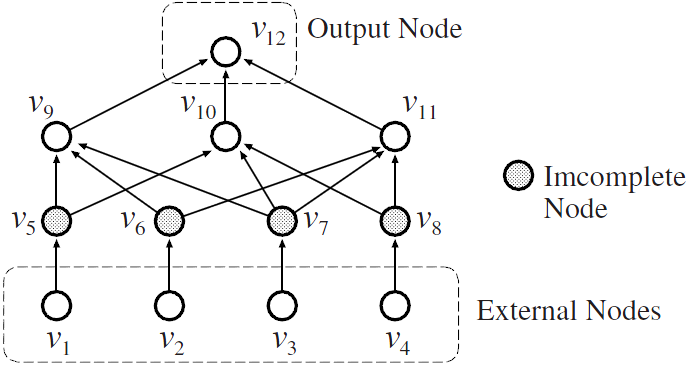
\includegraphics[width=0.6\textwidth]{Boolean.png}
\caption{Un r\'eseau bool\'een, selon les exp\'eriences, plusieurs exemples sont disponibles : $\mathbf{e}^i=\{v_1^i,v_2^i,v_3^i,v_4^i,v_{12}^i\}, i\in[1;n]$ avec $n$ le total d'exp\'eriences, car les fonctions bool\'eennes de $v_9\sim v_{11}$ sont d\'ej\`a connues, il reste donc \`a d\'eterminer celles de $v_5\sim v_8$}
\end{figure}
\subsection{Langage SBGN-AF}
Le SBGN-AF (System Biology Graphical Notation, Activity Flow en anglais) est un des formalismes standardis\'es principaux pour repr\'esenter les r\'eseaux de r\'egulation et les influences entre eux. Cette approche sert \`a trouver les bonnes fonctions bool\'eennes selon les hypoth\`eses. Le langage du SBGN-AF consiste d'un ensemble d'\'etiquettes, class\'e dans 5 groupes : \textit{n\oe uds d'activit\'e, unit\'es auxiliaires, n\oe uds de container, arcs de modulation et op\'erateurs logiques}.

Exemple : dans le Figure \ref{fig1},

N\oe uds d'activit\'e : $$activity(A_1), activity(A_2), activity(A_3), activity(A_4)$$
op\'erateurs logiques : $$or(lo_1), and(lo_2), not(lo_3)$$
arcs de modulation : $$input(A_1,lo_1), input(A_2, lo_1), input(lo_1,lo_2), input(lo_3, lo_2)$$
$$ stimulates(lo_2, A_4), inhibits(A_4, A_1)$$

\begin{figure}[ht]
\centering
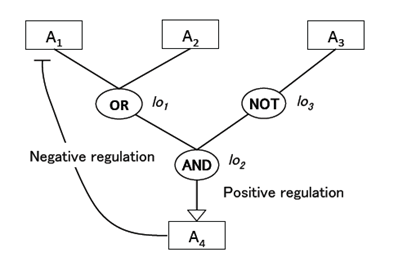
\includegraphics[width=0.5\textwidth]{SBGN-AF.png}
\caption{Exemple de r\'eseau SBGN-AF qui signifie $A_4=(A_1\lor A_2)\land\lnot A_3$ et $A_1=\lnot A_4$}
\label{fig1}
\end{figure}
Le raisonnement de compl\'etion est comme suit : 

\'Etant donn\'e un exemple $\mathbf{e}$, on cherche une hypoth\`ese $H$ par rapport aux connaissances existantes $B$ et $\mathbf{e}$, on en d\'eduit $B\land\lnot H\models\lnot \mathbf{e}$ et $B \not\models\lnot H$. En cons\'equence, $\lnot H$ est consid\'er\'ee comme une cons\'equence de $B\land\lnot \mathbf{e}$. Avec l'outil SOLAR, les hypoth\`eses sont trouv\'ees. C'est pour ceci cette m\'ethode est nomm\'ee ``Hypothesis finding'' \citep{Yamamoto2014,Nabeshima2010}.

C'est un raisonnement binaire appliquant sur les r\'eseaux bool\'eens, qui n'\'etudie pas les \'etats des \'el\'ements dans le syst\`eme, mais il nous inspire de renverser le lien causal entre les hypoth\`eses et les observations. (recherche des hypoth\`eses qui v\'erifient l'observation). Avant de parler du Process Hitting, une m\'ethode plus pr\'ecise poss\'edant plusieurs caract\'eristiques, nous aimerions pr\'esenter sa base : mod\`ele de Thomas.
\section{Mod\`ele de Thomas}
\'Etant un mod\`ele plus pr\'ecis que le r\'eseau bool\'een, le mod\`ele de Thomas contient plusieurs valeurs \`a un n\oe ud au lieu de deux, et il propose une description dynamique (attracteur) au lieu de fonctions bool\'eennes, qui donne la possibilit\'e de simuler les transitions des r\'eseaux biologiques.

Nous utilisons souvent les \'equations diff\'erentielles pour d\'ecrire la dynamique de chaque partie d'un RRB afin d'obtenir une s\'erie d'\'equations diff\'erentielles. A partir d'un RRB, on a une s\'erie d'\'equations diff\'erentielles lin\'eaires par morceaux \citep{filippov1960differential}. Pour simplifier l'analyse, ces \'equations sont consid\'er\'ees \'equivalentes \`a un ensemble des \'el\'ements discrets, qui change le probl\`eme en l'analyse d'un espace d'\'etats \citep{Glass1973}.

Selon Thomas, un RRB peut \^etre repr\'esent\'e formellement et qualitativement par un graphe. (e.g. La concentration d'un certain mati\`ere est class\'ee par plusieurs niveaux, mais les \'ecarts entre niveaux ne sont pas forc\'ement \'egaux)

\begin{Def}[Graphe de r\'egulation]
Un graphe de r\'egulation est un graphe orient\'e \'etiquet\'e, not\'e $G = (V, E)$, chaque sommet $v \in V$ est une variable discr\`ete avec son seuil $b_v\in \mathbb{N}$ inf\'erieur \`a son degr\'e sortant. Chaque arc est \'etiquet\'e par un couple $(t_{\rm{uv}}, \alpha_{\rm{uv}})$, dont $t_{\rm{uv}}$ est un entier compris entre $1$ et $b_u$, appel\'e le seuil qualitatif et o\`u $\alpha_{uv} \in \{+ ,-\}$ est la signe de r\'egulation. 
\end{Def}
Toutes r\'egulations sont consid\'er\'ees comme effectives, i.e. lorsque $\alpha_{uv}=+, u \geq t_{uv}$ veut dire $u$ active $v$ et $u < t_{uv}$ veut dire $u$ inhibe $v$, vice versa pour le cas $\alpha_{uv}=-$.
\begin{Def}[\'Etat qualitatif]
\'Etant donn\'e $G = (V, E)$ un graphe de r\'egulation, un \'etat qualitatif de $G$ est un vecteur $q=(q_v)_{v \in V}$ tel que pour tout $v \in V$, $q_v \in \{0, 1, ... , b_v\}$ . L'ensemble $Q$ des \'etats de $G$ est alors d\'efini comme $Q=\prod_{v \in V}\{0, 1, ..., b_v\}$.
\end{Def}
\begin{figure}[ht]
\begin{minipage}{0.45\linewidth}
\centering
\begin{tikzpicture}
\draw[->] (-5pt,5pt) .. controls (-1,1)  and (-1,-1) .. (-5pt,-5pt);
\node at (0,0) {u};
\node at (2.2,0) {v};
\node at (-1.5,0){$(2,+)$};
\node at (1,1.1){$(1,+)$};
\node at (1,-1.1){$(1,-)$};
\draw[->] (5pt,5pt) .. controls (0.67,1) and (1.33,1) .. (2,5pt);
\draw[->] (2,-5pt) .. controls  (1.33,-1)and (0.67,-1) .. (5pt,-5pt);
\end{tikzpicture}
\caption{(a)}
\end{minipage}
\begin{minipage}{0.45\linewidth}
\centering
\begin{tikzpicture}[line width=1pt]
\draw[->] (0,0) -- (3.5,0);
\draw[->] (0,0) -- (0,2.5);
\draw[step=1] (0,0) grid (3,2);
\node at (3.5,0)[anchor=north]{\small u};
\node at (0,2.5)[anchor=east]{\small v};
\foreach \x in {0,1,2}
\node at ($(\x,0)+(0.5,0)$)[anchor=north] {\small $\x$};
\foreach \y in {0,1}
\node at ($(0,\y)+(0,0.5)$)[anchor=east] {\small $\y$};
\foreach \x in {0,1,2}
\foreach \y in {0,1}
\node at ($(\x,\y)+(0.5,0.5)$){\small $(\x,\y)$};
\node at (1,0)[anchor=north]{$t_{uv}$};
\node at (2,0)[anchor=north]{$t_{uu}$};
\node at (0,1)[anchor=east]{$t_{vu}$};
\end{tikzpicture}
\caption{(b)}
\end{minipage}
\caption{(a) Un graphe de r\'egulation (b) L'espace d'\'etats de ce graphe de r\'egulation}\label{figres}
\end{figure}
\begin{Def}[Ressource]
$G=(V,E)$ est un graphe de r\'egulation, $v\in V$et $q\in Q$. L'ensemble $\omega_v(q)$ de ressources de $v$ \`a l'\'etat $q$ est le sous-ensemble de $G^-(v)$ :
$$\omega_v(q)=\{u\in G^-(v)\mid(q_u\geq t_{uv}\ et\ \alpha_{uv}=+)\ ou\ (q_u\leq t_{uv}\ et\ \alpha_{uv}=-)\}$$
\end{Def}
\`A l'\'etat $q$, l'\'evolution de la variable $v$ d\'epend de ses ressources $\omega_v(q)$. Il reste \`a d\'efinir la direction d'\'evolution. Le param\`etre $K_{v,\omega_v(q)}$ est appel\'e l'attracteur de $v$ lorsque l'ensemble de ressources est $\omega_v(q)$. Il donne la tendance d'\'evolution de $v$:
\begin{itemize}
\item si $q_v<K_{v,\omega_v(q)}$, alors $v$ va augmenter
\item si $q_v=K_{v,\omega_v(q)}$, alors $v$ va rester invariant
\item si $q_v>K_{v,\omega_v(q)}$, alors $v$ va diminuer
\end{itemize}
Les valeurs diff\'erentes des attracteurs sont possibles, les combinaisons d'attracteurs sont appel\'ees \textit{mod\`eles}.
\begin{Def}[Mod\`ele]
$G=(V,E)$ est un graphe de r\'egulation. Un mod\`ele de $G$, not\'e par $M(G)$, est un groupe de nombres naturels $K_{v,\omega}$ index\'es par la par l'ensemble des couple $(v,\omega)$ tel que :
\begin{itemize}
\item $v\in V$
\item $\omega \subseteq G^-(v)$
\item $K_{v,\omega}\leq b_v$ 
\end{itemize}
\end{Def}
Il exige souvent que :
$K_{v,\omega} \leq K_{v,\omega'}$ pour tous les $v\in V$ et pour tous les $\omega, \omega'\subseteq G$ tels que $\omega\subseteq\omega'$ (Les contraintes de Snoussi) \citep{Richard2006}. 

\begin{table}[ht]\large
\centering
\begin{tabular}{l|l l|l l|c c}
Mod\`ele & u & v &\multicolumn{2}{|c|}{Attracteurs}&\multicolumn{2}{|c}{Tendances}\\
\hline
$K_{u,\{\}}=0$&0&0&$K_{u,\{v\}}=2$&$K_{v,\{\}}=0$&$\nearrow$&$\to$\\
$K_{u,\{u\}}=2$&0&1&$K_{u,\{\}}=0$&$K_{v,\{\}}=0$&$\to$&$\searrow$\\
$K_{u,\{v\}}=0$&1&0&$K_{u,\{v\}}=2$&$K_{v,\{u\}}=1$&$\nearrow$&$\nearrow$\\
$K_{u,\{u,v\}}=2$&1&1&$K_{u,\{\}}=0$&$K_{v,\{u\}}=1$&$\nearrow$&$\to$\\
$K_{v,\{\}}=0$&2&0&$K_{u,\{u,v\}}=2$&$K_{v,\{u\}}=1$&$\to$&$\nearrow$\\
$K_{u,\{u\}}=1$&2&1&$K_{u,\{u\}}=2$&$K_{v,\{u\}}=1$&$\to$&$\to$
\end{tabular}
\caption{Un mod\`ele possible du graphe de r\'egulation du Figure \ref{figres}. Ce tableau montre les attracteurs correspondant \`a chaque \'etat qui est d\'eduit du mod\`ele.}\label{tab1}
\end{table}
\subsection{Boucles de RRB}
Lorsqu'on analyse un RRB, on fait souvent attention aux boucles positives et boucles n\'egatives. Une boucle est positive (resp. n\'egative) si dans son circuit le nombre des signes de r\'egulation n\'egative est pair (resp. impair). Une boucle positive active ou inhibe toujours les variables dans le circuit, qui atteint finalement son seuil ou le minimum permis afin de rester toujours disponible. Un boucle n\'egative active (resp. inhibe) toutes les variables lorsque cette variable atteint un assez bas (resp. haut) niveau, afin de stabiliser le syst\`eme en comportant comme l'oscillation ou la multistationnarit\'e \citep{Thomas1978}.
\subsection{Dynamique des mod\`eles}
L'approche classique pour d\'ecrire la dynamique de mod\`eles est de d\'efinir l'\'etat du syst\`eme au moment t+1 \`a partir de l'\'etat du moment t. L'approche synchrone est de consid\'erer que l'\'etat suivant est l'attracteur de l'\'etat actuel : si $q$ est l'\'etat actuel alors $q'=(K_{v,\omega_v(q)})_{v\in V}$ est le prochain \'etat, c'est-\`a-dire il y a une transition de $q$ \`a $q'$. Cette approche entra\^ine des probl\`emes graves, principalement \`a cause des propri\'et\'es d\'eterministes \citep{Richard2006}.

Alors ces probl\`emes nous m\`ene \`a une nouvelle approche :
\begin{Def}[graph d'\'etat asynchrone]
$G=(V,E)$ est un graphe de r\'egulation et $M(G)$ est un mod\`ele de $G$. Le graphe d'\'etat asynchrone est un graphe orient\'e dont l'ensemble des sommets est l'ensemble $Q$ des \'etats de $G$, tel qu'il existe un arc de $q$ \`a $q'$ si :
\begin{itemize}
\item Pour tous les variables $v\in V$, $q_v=q'_v=K_{v,\omega_v(q)}$ ou
\item Il existe une variable $v\in V$ telle que :
\begin{itemize}
\item Pour toute variable $u\neq v$, $q_u=q'_u$ et
\item $q_v<K_{v,\omega_v(q)}$ et $q'_v=q_v+1$ ou $q_v>K_{v,\omega_v(q)}$ et $q'_v=q_v-1$
\end{itemize}
\end{itemize}
\end{Def} 
\begin{figure}[ht]
\begin{minipage}{0.45\linewidth}
\centering
\begin{tikzpicture}[line width=1pt]
\draw[->] (0,0) -- (3.5,0);
\draw[->] (0,0) -- (0,2.5);
\draw[step=1] (0,0) grid (3,2);
\node at (3.5,0)[anchor=north]{\small u};
\node at (0,2.5)[anchor=east]{\small v};
\foreach \x in {0,1,2}
\node at ($(\x,0)+(0.5,0)$)[anchor=north] {\small $\x$};
\foreach \y in {0,1}
\node at ($(0,\y)+(0,0.5)$)[anchor=east] {\small $\y$};
\node at (1,0)[anchor=north]{$t_{uv}$};
\node at (2,0)[anchor=north]{$t_{uu}$};
\node at (0,1)[anchor=east]{$t_{vu}$};
\draw[->] (0.5,1.4) -- (0.5,0.6);
\draw[->] (1.4,1.5) -- (0.6,1.5);
\draw[dotted,->] (0.6,0.5) -- (2.4,0.5);
\draw[dashed,->] (1.6,0.6) -- (2.4,1.4);
\draw[->] (2.5,0.6) -- (2.5,1.4);
\draw[->] (2.6,1.4) arc (-90:240:0.25);
\end{tikzpicture}
\caption{(a) synchrone}
\end{minipage}
\begin{minipage}{0.45\linewidth}
\centering
\begin{tikzpicture}[line width=1pt]
\draw[->] (0,0) -- (3.5,0);
\draw[->] (0,0) -- (0,2.5);
\draw[step=1] (0,0) grid (3,2);
\node at (3.5,0)[anchor=north]{\small u};
\node at (0,2.5)[anchor=east]{\small v};
\foreach \x in {0,1,2}
\node at ($(\x,0)+(0.5,0)$)[anchor=north] {\small $\x$};
\foreach \y in {0,1}
\node at ($(0,\y)+(0,0.5)$)[anchor=east] {\small $\y$};
\node at (1,0)[anchor=north]{$t_{uv}$};
\node at (2,0)[anchor=north]{$t_{uu}$};
\node at (0,1)[anchor=east]{$t_{vu}$};
\draw[->] (0.5,1.4) -- (0.5,0.6);
\draw[->] (1.4,1.5) -- (0.6,1.5);
\draw[->] (0.6,0.5) -- (1.4,0.5);
\draw[->] (1.6,0.5) -- (2.4,0.5);
\draw[->] (1.5,0.6) -- (1.5,1.4);
\draw[->] (2.5,0.6) -- (2.5,1.4);
\draw[->] (2.6,1.4) arc (-90:240:0.25);
\end{tikzpicture}
\caption{(b) asynchrone}
\end{minipage}
\caption{(a) et (b) montre respectivement la dynamiques synchrone et la dynamique asynchrone du mod\`ele de tableau \ref{tab1}. Les attracteurs sont pareils mais les chemins sont diff\'erents : le graphe d'\'etat asynchrone contient un circuit $(0,0)\to(1,0)\to(1,1)\to(0,1)\to(0,0)$, qui est absent dans l'approche synchrone. Nous pouvons voir que dans le figure (a) il y a au plus une seule possibilit\'e dans tous les \'etats, c'est bien la d\'efinition de d\'eterminisme, et que dans le figure (b) il y a 2 chemins dans l'\'etat $(u,v)=(1,0)$.}
\end{figure}

\section{Process Hitting}
Inspir\'e par le graphe d'\'etat asynchrone, le Process Hitting donne la possibilit\'e de simuler le syst\`eme biologique pas \`a pas et de fa\c con encore plus pr\'ecise, poss\'edant des caract\'eristiques stochastiques et temporis\'ees \citep{pauleve2011refining}.
\subsection{Concepts fondamentaux}
\begin{Def}[Process Hitting]
Un Process Hitting $PH$ est constitu\'e d'un triplet $(\Sigma, L, \mathscr{H})$ avec:

--$\Sigma=\{a,b,...\}$ est l'ensemble fini des sortes

--$L=\prod_{a\in\Sigma}{L_a}$ est un ensemble d'\'etats avec $L_a=\{a_0,...a_{l_a}\}$ l'ensemble fini des processus de la sorte $a\in\Sigma$ et $l_a$ est un entier positif satisfaisant:
$$a\neq b\to \forall(a_i,b_j)\in L_a\times L_b,a_i\neq b_j$$
L'ensemble fini d'actions est d\'efini comme suit :
$$\mathscr{H}=\{a_i\to b_j\Rsh b_k\mid(a,b)\in\Sigma^2,(a_i,b_j,b_k)\in L_a\times L_b\times L_b,b_j\neq b_k, a=b\to a_i=b_j\}$$
$a_i, b_j, b_k$ sont not\'es respectivement $hitter(h)$, $target(h)$ et $bounce(h)$ d'une action $h$.
\end{Def}
On note l'ensemble de tous les processus ${\bf Proc}=\{a_i\mid a\in\Sigma \land a_i\in L_a\}$.

On note la sorte d'un processus $a_i$ par $\Sigma(a_i)=a$ et 
$\Sigma(h)=\{\Sigma(hitter(h)),\Sigma(target(h))\}$
pour noter l'ensemble des sortes pr\'esentes dans une action $h\in H$. \'Etant donn\'e un \'etat $s\in L$, le processus de la sorte $a\in\Sigma$ pr\'esent dans $s$ est not\'e par $s[a]$, qui est la i-\`eme coordonn\'ee de l'\'etat $s$. On a \'egalement les notations suivantes:

$$	\text{si } a_i\in L_a, a_i\in s\xLeftrightarrow{\Delta}[a]=a_j \text{ et si } ps\in p({\bf Proc}), ps \subseteq s\xLeftrightarrow{\Delta}\forall a_i\in ps,a_i\in s$$

Une action $h= \acm{a_i}{b_j}{b_k} \in \mathscr{H}$ est dite jouable dans $s\in L$ si et seulement si $s[a]= a_i$ et $s[b]= b_j$. Dans ce cas-l\`a, $(s\cdot h)$ repr\'esente l'\'etat issu de l'ex\'ecution de l'action $h$ dans s, i.e. $c[b]= b_k$ et \'evidemment que $\forall c\in \Sigma,c\neq b,(s\cdot h)[c]=s[c]$ , et que $((s\cdot h)\cdot h')= (s\cdot h\cdot h')$.
\begin{Def}[Contexte]
Un contexte $\varsigma$ associe chaque sorte dans $\Sigma$ \`a un sous-ensemble non-vide de ses propres processus : $\forall a \in \Sigma, c[a]\subseteq L_a\land c[a]\neq \varnothing$.
\end{Def}

On note l'ensemble des contextes par {\bf Ctx}.
\begin{Def}[Sc\'enario]
Etant donn\'e un Process Hitting $PH=(\Sigma, L, \mathscr{H})$, un sc\'enario $\delta=h_1:\,:...:\,:h_n$ est une s\'equence des actions dans $H$ qui peuvent \^etre tir\'ees l'une par l'autre. %$n\in\uppercase\expandafter{\romannumeral2}^\delta$
\end{Def}
L'ensemble de tous les sc\'enarios est not\'e par {\bf Sce}.
\begin{Def}[Action li\'ee]
Pour un certain processus $a_i$, une action avec son target $a_i$ est dite li\'ee \`a $a_i$, qui prend la forme \ac{b_k}{a_j}{a_i}.
\end{Def}
L'ensemble des actions li\'ees du processus $p$ est not\'e $\mathbf{LA}(p)$.

\'Etant donn\'e une s\'equence des actions, on utilise $fst_a (A)$ pour noter le premier processus de la sorte a pr\'esent dans la s\'equence, et $last_a (A)$ pour noter le dernier processus.

$$fst_a(A)\triangleq 
\begin{cases}
\varnothing &\text{si }a \notin\Sigma(A)\\
             hitter(A_m) &\text{si }m=min\{n \in \text{\uppercase\expandafter{\romannumeral2}}^A\mid a \in \Sigma(A_n)
             \land\Sigma(hitter(A_m))=a\}\\ 
             target(A_m) &\text{si }m=min\{n \in \text{\uppercase\expandafter{\romannumeral2}}^A\mid a \in \Sigma(A_n)
             \land\Sigma(target(A_m))=a\}
\end{cases}
$$

$$last_a(A)\triangleq 
\begin{cases}
\varnothing &\text{si }a \notin\Sigma(A)\\
             bounce(A_m) &\text{si }m=max\{n \in \text{\uppercase\expandafter{\romannumeral2}}^A\mid a \in \Sigma(A_n)
             \land\Sigma(bounce(A_m))=a\}\\ 
             hitter(A_m) &\text{si }m=max\{n \in \text{\uppercase\expandafter{\romannumeral2}}^A\mid a \in \Sigma(A_n)
             \land\Sigma(hitter(A_m))=a\}\\  
\end{cases}
$$

O\`u $\text{\uppercase\expandafter{\romannumeral2}}^A\triangleq\{1,\ldots,|A|\}$ est l'ensemble des indexes de $A$.

Un sc\'enario $\delta\in{\bf Sce}$ est dit jouable dans le contexte $\varsigma$ si et seulement si $support(\delta)\subseteq\varsigma$. L'ex\'ecution de $\delta$ dans $\varsigma$ est not\'e par $\varsigma$ o\`u $\varsigma\cdot\delta=\varsigma\cap end(\delta)$.

Les fonctions $support(\delta)$ et $end(\delta)$ donnent respectivement le premier et le dernier processus de chaque sorte pendant la simulation:

\begin{equation}
\begin{aligned}
support(\delta)&\triangleq\{p\in {\bf Proc} \mid \Sigma(p)\in \Sigma(\delta)\land p= fst_{\Sigma(p)}  (\delta)\}\\
end(\delta)&\triangleq\{p\in{\bf Proc} \mid\Sigma(p)\in \Sigma(\delta)\land p= last_{\Sigma(p)}  (\delta)\}\nonumber
\end{aligned}
\end{equation}
Exemple : 
\begin{figure}[ht]
\centering
\begin{tikzpicture}%[font=\scriptsize]
%\path[use as bounding box] (0,-1) rectangle (4,4);
%{left, right, top, bottom}
\TSort{(0,0)}{a}{2}{l}
\TSort{(4,0)}{b}{3}{l}
\TSort{(8,0)}{d}{3}{r}
\TSort{(3,-2)}{c}{2}{b}
\THit{a_1}{}{b_1}{.west}{b_0}
\THit{a_0}{}{c_0}{.north}{c_1}
\THit{b_1}{}{a_0}{.east}{a_1}
\THit{c_1}{out=120,in=255}{b_0}{.west}{b_1}
\THit{b_0}{}{d_0}{.west}{d_1}
\THit{b_1}{}{d_1}{.west}{d_2}
\THit{b_2}{bend right=45,in=-30}{d_0}{.east}{d_2}
\THit{d_1}{}{b_0}{.north east}{b_2}
\THit{c_1}{bend right=150,out=-90,in=-90}{d_1}{.south east}{d_0}

\path[bounce,bend right]
\TBounce{b_1}{}{b_0}{.north}
\TBounce{a_0}{}{a_1}{.south}
\TBounce{d_0}{}{d_2}{.south}
\TBounce{b_0}{}{b_2}{.south}
;
\path[bounce,bend left]
\TBounce{d_0}{}{d_1}{.south}
\TBounce{b_0}{}{b_1}{.south}
\TBounce{c_0}{}{c_1}{.west}
\TBounce{d_1}{}{d_2}{.south}
\TBounce{d_1}{}{d_0}{.north}
;
\path[bounce,bend left]
;
\TState{a_0,b_1,c_0,d_0}
\end{tikzpicture}
\caption{Exemple de Process Hitting}\label{phex}
\end{figure}
Le Figure repr\'esente un Process Hitting $(\Sigma, L, \mathscr{H})$ o\`u 
$$\Sigma=\{a,b,c,d\}$$
$$L=\{a_0,a_1 \}\times\{b_0,b_1,b_2 \}\times\{c_0,c_1 \}\times\{d_0,d_1,d_2\}$$
\begin{align*}
\mathscr{H}=\{&\acm{a_0}{c_0}{c_1},\acm{a_1}{b_1}{b_0},\acm{c_1}{b_0}{b_1},\acm{b_1}{a_0}{a_1},\acm{b_0}{d_0}{d_1},\\
&\acm{b_1}{d_1}{d_2},\acm{d_1}{b_0}{b_2},\acm{c_1}{d_1}{d_0},\acm{b_2}{d_0}{d_2}\}
\end{align*}
$$\mathbf{LA}(d_2)=\{\acm{b_1}{d_1}{d_2}, \acm{b_2}{d_0}{d_2}\},\ \mathbf{LA}(a_0)=\varnothing$$
\'Etant donn\'e le contexte
$$\varsigma=\langle a_0,b_0,b_1,c_0,d_1\rangle$$
Avec
$$support(\delta)=\langle a_0,b_1,c_0,d_1\rangle$$
Et le sc\'enario
$$\delta=a_0\to c_0\Rsh c_1:\,:b_1\to a_0\Rsh a_1:\,:b_1\to d_1\Rsh d_2$$
Si $\delta$ est jouable dans $\varsigma$, on a :
$$end(\delta)=c\cdot\delta\langle a_0,b_0,b_1,c_0,d_1\rangle\cap\{a_1,b_1,c_1,d_2\}=\langle a_1,b_1,c_1,d_2\rangle$$

\subsection{Outil Pint}
{\large{P}}INT est un ensemble de commandes en ligne, qui impl\'emente les analyses vari\'ees de Process Hitting. Parmi les commande en ligne, \texttt{ph-reach} sert \`a l'accessibilit\'e et \texttt{ph-exec} sert \`a la simulation d'\'evolution d'un r\'eseau Process Hitting, qui sont importants dans cette recherche. Les donn\'ees de r\'eseaux Process Hitting sont enregistr\'ees dans un fichier \texttt{.ph}. Voici l'exemple d'un fichier \texttt{.ph} \citep{Pauleve2014} :
\vspace{0.2cm}
\hrule
\begin{verbatim}
(* Declaration of sorts *)
process a 1 process b 2 process c 1 process d 2

(*Definition of actions*)
a 0 -> c 0 1 a 1 -> b 1 0 c 1 -> b 0 1
b 1 -> a 0 1 b 0 -> d 0 1 b 1 -> d 1 2
d 1 -> b 0 2 c 1 -> d 1 0 b 2 -> d 0 2

initial_state 
a 1, b 0, c 0,d 1
\end{verbatim}
\hrule
En ex\'ecutant \texttt{ph-reach -i <filename> d 2}, on a une valeur retourn\'ee \texttt{false} impliquant que le processus $d_2$ n'est pas accessible.

En ex\'ecutant \texttt{ph-exec -i <filename> 10}, on obtient les fichiers des informations de la stimulation par \'etape dans une p\'eriode de 10 unit\'es de temps.

\chapter{Causalit\'e locale}
Il arrive souvent que nous nous int\'eressons \`a l'accessibilit\'e d'un certain processus, mais la complexit\'e d'un raisonnement exhaustive est assez importante (comme montr\'e dans la Section 1.4.3, l'explosion d'espace d'\'etats). C'est pour ceci nous avons besoin d'une structure pour raisonner de fa\c con non-exhaustive et assez pr\'ecise.

Selon \textit{Loïc Paulev\'e} \citep{Pauleve2013}, en analysant s\'epar\'ement(e.g. localement) et statiquement les processus, il est possible de r\'eduire la complexit\'e de calcul par rapport au calcul exhaustif.

\'Etant donn\'e un Process Hitting $(\Sigma,L,\mathscr{H})$, pour tout $a\in \Sigma$, $S(a)=[1;l_a]$, est l'ensemble fini des \'etats locaux de l'automate $a$; $S=\prod_{a\in\Sigma}[1;l_a]$ est l'ensemble fini des \'etats globaux.

On note l'ensemble des \'etats locaux ${\bf LS}\triangleq\{a_i\mid a\in\Sigma\land i\in[1;l_a]\}$

\begin{Def}[Accessibilit\'e de processus]
\'Etant donn\'e un Process Hitting $(\Sigma, L, \mathscr{H})$ et un contexte $\varsigma$, l'\'etat local $a_j\in\mathbf{LS}$ est accessible \`a partir de $\varsigma$ si et seulement si $\exists s_0,\cdots,s_m\in S$ tel que $\forall a\in\Sigma,s_0(a)\in\varsigma(a)$, et $s_0\to\cdots\to s _m$, et $s_m(a)=j$.
\end{Def}
Dans une sorte $a$, l'accessibilit\'e globale de $a_j$ \`a partir de $a_i$ peut \^etre repr\'esent\'ee par celle de $a_j$ \`a partir d'un \'etat local $a_i\in \varsigma(a)$. Cette accessibilit\'e locale se r\'ef\`ere \`a un objectif not\'e $a_i\Rsh^* a_j$.
\begin{Def}[Objectif]
L'accessibilit\'e d'un \'etat local $a_j$ depuis $a_i$ est appel\'e un objectif not\'e $a_i\to a_j$. L'ensemble de tous les objectifs est d\'efini comme ${\bf Obj}\triangleq\{a_i\to a_j \mid(a_i,a_j)\in {\bf LS\times LS}\}$
\end{Def}
\'Etant donn\'e un objectif $P=a_i\to^*a_j\in {\bf Obj}$, on d\'efinit $\mathsf{sol}(P)$ comme la causalit\'e locale de $P$ : chaque \'el\'ement $ls\in \mathsf{sol}(P)$ est un sous-ensemble d'\'etats locaux, r\'ef\'er\'e \`a une solution (locale) de $P$, qui sont des fois plus faciles \`a obtenir que l'accessibilit\'e de $a_j$. $\mathsf{sol}(P)$ est solide si la d\'esactivation d'au moins un \'etat local dans chaque solution rend l'accessibilit\'e de $a_j$ impossible depuis tout \'etat global contenant $a_i$. Remarquons que si $\mathsf{sol}(P)=\{ls^1,\ldots,ls^m\}$ est solide, alors $\mathsf{sol}'(P)=\{ls^1,\ldots,ls^m\}$ est aussi solide. $\mathsf{sol}(a_i\to^*a_j)=\varnothing$ implique que $a_j$ ne peut pas \^etre atteint et $\forall a_i\in {\bf LS}, \mathsf{sol}(a_i\to^*a_j)\triangleq\{\varnothing\}$
\begin{Def}[Solution]
${\bf Obj}\to\mathcal{P}(\mathcal{P}(\mathbf{LS}))$ est un mappage d'objectifs \`a ensembles d'ensembles des \'etats locaux tels que $\forall P\in \mathbf{Obj},\forall ls \in \mathsf{sol}(P), \nexists ls'\in \mathsf{sol}(P), ls\neq ls'$ tel que $ls'\subset ls$. L'ensemble de ces mappages est not\'e $\mathbf{Sol}\triangleq\{\langle P,ls\rangle\mid ls\in \mathsf{sol}(P)\}$.
\end{Def}
\section{Graphe de causalit\'e locale}
Avec les d\'efinitions pr\'eliminaires, nous pouvons maintenant construire une structure abstraite sans toucher les \'etats globaux afin de r\'eduire la complexit\'e du calcul de l'accessibilit\'e d'un certain processus \citep{Pauleve2013}.
\begin{Def}[GLC]
\'Etant donn\'e un contexte $\varsigma$ et un ensemble d'\'etats locaux $\omega\subseteq \mathbf{LS}$, le Graphe de Causalit\'e Locale (Graph of Local Causality en anglais) $\mathcal{A}^\omega_\varsigma\triangleq(V^\omega_\varsigma,E^\omega_\varsigma)$, avec $V^\omega_\varsigma\subseteq \mathbf{LS\cup Obj\cup Sol}$ et $E^\omega_\varsigma\subseteq V^\omega_\varsigma\times V^\omega_\varsigma$ est la plus petite structure satisfaisant :
\begin{equation}
\centering
\begin{aligned}
\omega&\subseteq V^\omega_\varsigma\\
a_i\in V^\omega_\varsigma\cap\mathbf{LS}&\Leftrightarrow\{(a_i,a_j\to^*a_i)\mid a_j\in\varsigma\}\subseteq E^\omega_\varsigma\\
a_i\to^*a_j\in V^\omega_\varsigma\cap\mathbf{Obj}&\Leftrightarrow\{(a_i\to^*a_j,\langle a_i\to^*a_j,ls\rangle)\mid\langle a_i\to^*a_j,ls\rangle\in \mathbf{Sol}\}\subseteq E^\omega_\varsigma\\
\langle P,ls\rangle\in V^\omega_\varsigma\cap\mathbf{Sol}&\Leftrightarrow\{(\langle P,ls\rangle,a_i)\mid a_i\in ls\}\subseteq E^\omega_\varsigma\nonumber
\end{aligned}
\end{equation}
\end{Def}
Le graphe de causalit\'e locale (GLC, graph of local causality en anglais) r\'ealise cette raisonnement r\'ecursif \`a partir d'un ensemble donn\'e des \'etats locaux $\omega\in\mathbf{LS}$ en reliant chaque \'etat local $a_j$ \`a tous les objectifs $a_i\Rsh^*a_j$, $a_i\in\varsigma(a)$, et en reliant chaque objectif $P$ \`a leurs solutions $\langle P,ls\rangle\in\mathbf{Sol}$, et en reliant toutes les solutions $\langle P,ls\rangle$ \`a leurs \'etats locaux $b_k\in ls$. Un GLC est dit valide si $\mathsf{sol}$ est solide pour tous les objectifs apparus.
\section{Sur-approximation}
Avant d'entrer dans cette partie, il y a quelques notions importantes :  
\begin{Def}[S\'equence de bounce(\textbf{BS})]
La s\'equence de bounces $\zeta$ est une s\'equence des actions telle que $\forall n\in\text{\uppercase\expandafter{\romannumeral2}}^\zeta,n<|\zeta|,bounce(\zeta_n)=target(\zeta_{n+1})$. On l'utilise pour d\'ecrire l'ensemble des s\'equence de bounces, et \textbf{BS}(P) pour noter l'ensemble de s\'equence de bounces qui r\'esolvent l'objectif $P$ :
\begin{equation}
\begin{aligned}
\mathbf{BS}(a_i\to^*a_j)\{\zeta\in\mathbf{BS}\mid &\ target(\zeta_1)=a_i\land bounce(\zeta_{|\zeta|})=a_j\\
&\land\forall m,n\in\text{\uppercase\expandafter{\romannumeral2}}^\zeta,n>m,bounce(\zeta_n)\neq target(\zeta_m)\}
\end{aligned}
\nonumber
\end{equation}
\end{Def}
Bien entendu, on a 
$$\mathbf{BS}(a_i\to^*a_i)=\{\varepsilon\},$$
et
$$\mathbf{BS}(a_i\to^*a_j)=\varnothing$$
s'il est impossible d'acc\'eder de $a_i$ \`a $a_j$.

Avec la d\'efinition de s\'equence de bounce, on peut maintenant d\'efinir $\mathbf{BS}^\wedge$ qui repr\'esente la liste de processus n\'ecessaire pour que cet objectif soit r\'ealisable.
\begin{Def}[$\mathbf{BS}^\wedge:\mathbf{Obj}\mapsto\mathcal{P}(\mathbf{Proc})$]
$$\mathbf{BS}^\wedge(P)\triangleq\{\zeta^\wedge\mid\zeta\in\mathbf{BS}(P)\land\nexists\zeta'\in\mathbf{BS}(P),\zeta'^\wedge\subsetneq\zeta^\wedge\}$$ o\`u $\zeta^\wedge\triangleq\{hitter(\zeta_n)\mid n\in\text{\uppercase\expandafter{\romannumeral2}}^\zeta\land\Sigma(hitter(\zeta_n))\neq\Sigma(P)\}$
\end{Def}
Exemple : 

Dans le Figure \ref{phex}, pour r\'ealiser l'objectif $b_1\to^*b_2$, il faut tirer successivement les actions \ac{a_1}{b_1}{b_0} et \ac{d_1}{b_0}{b_2}, c'est exactement $\mathbf{BS}^\wedge(b_1\to^*b_2)=\{\{a_1,d_1\}\}$.

La sur-approximation s'applique le GLC qui est une condition suffisante de l'accessibilit\'e d'un certain processus. Sa structure abstraite est not\'ee $\mathcal{A}^\omega_\varsigma$ \citep{Pauleve2012} : 

\begin{Def}[$\mathcal{A}^\omega_\varsigma$]
\'Etant donn\'e un contexte $\varsigma$ et une s\'equence d'objectifs,
$$\mathcal{A}^\omega_\varsigma=(Req^\omega_\varsigma,Sol^\omega_\varsigma,Cont^\omega_\varsigma)$$
o\`u $Req^\omega_\varsigma$, $Sol^\omega_\varsigma$ et $Cont^\omega_\varsigma$ sont d\'efinis comme suit :
\begin{equation}
\begin{aligned}
Req^\omega_\varsigma\triangleq\{(a_i,a_j\to^*a_i)\in\mathbf{Proc\times Obj}\mid a_j\in \varsigma[a]\land(&\exists(P,ps)\in Sol^\omega_\varsigma,a_i\in ps\\
&\lor\exists n\in\text{\uppercase\expandafter{\romannumeral2}}^\omega,bounce(\omega)=a_i)\}
\end{aligned}
\nonumber
\end{equation}
$$Sol^\omega_\varsigma\triangleq\{(P,ps)\in\mathbf{Obj\times \mathcal{P}(Proc)}\mid \exists(a_i,P)\in Req^\omega_\varsigma\land ps\in\mathbf{BS}^\wedge(P)\}$$
$$Cont^\omega_\varsigma\triangleq\{(P,Q)\in\mathbf{Obj\times Obj}\mid \exists(P,ps)\in Sol^\omega_\varsigma\land Q\in minCont_\varsigma(P)\}$$
\end{Def}
o\`u

\begin{Def}[$minCont_\varsigma:\mathbf{Obj}\mapsto\mathcal{P}(\mathbf{Obj})$]
$$minCont_\varsigma(^\bigstar\to^*a_j)\triangleq\{a_k\to^*a_j\mid a_k\neq a_j\land\forall a_i\in\varsigma[a],a_k\in minCont_\varsigma^{Obj}(a,a_i\to^*a_j)\}$$
$minCont_\varsigma^{Obj}:\Sigma\times\mathbf{Obj\mapsto\mathcal{P}(Proc)}$

$$minCont_\varsigma^{Obj}(a,P)\triangleq
\begin{cases}
\varnothing&\text{si }\mathbf{BS}^\wedge(P)=\varnothing\\
\{p\in \mathbf{Proc}\mid \forall ps\in\mathbf{BS}^\wedge(P),&\\
          \exists q\in ps,p\in minCont_\varsigma^{Proc}(a,q)\} &\text{sinon}
\end{cases}
$$

$minCont_\varsigma^{Obj}:\Sigma\times\mathbf{Obj\mapsto\mathcal{P}(Proc)}$

$$minCont_\varsigma^{Proc}(a,b_i)\triangleq
\begin{cases}
\{b_1\}                                                    &\text{si }a=b\\
\{p\in     \mathbf{Proc}\mid \forall b_j\in\varsigma[b],&\\
           p\in ps,p\in minCont_\varsigma^{Obj}(a,b_j\to^*b_i)\} &\text{sinon}
\end{cases}
$$
\end{Def}
o\`u $\bigstar$ signifie un processus de certaine sorte \`a niveau quelconque.

Dans le Figure \ref{overapp}, la structure abstraite $\mathcal{A}^\omega_\varsigma$ commence par un n\oe ud de processus (carr\'e), il relie les objectifs associ\'es et chaque objectif relie un n\oe ud de solution (cercle), enfin, les n\oe uds de solutions relient ses processus composants. Les $\perp$ signifient l'inaccessibilit\'e de cette branche \citep{Pauleve2012}.
\begin{figure}[ht]
\centering
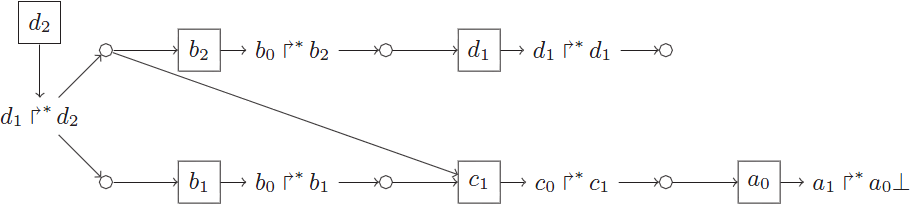
\includegraphics[scale=0.6]{overapp.png}
\caption{La structure abstraite $\mathcal{A}^\omega_\varsigma$ de l'exemple de Process Hitting dans le Figure \ref{phex} avec $\omega=d_1\Rsh^*d_2$ et $\varsigma=\langle a_1,b_0,c_0,d_1\rangle$ , cet objectif n'est pas r\'ealisable.}\label{overapp}
\end{figure}
\section{Sous-approximation}
De fa\c con analogue, la sous-approximation est bas\'ee sur la structure abstraite $\lceil\mathcal{B}^\omega_\varsigma\rceil$ : 

\begin{Def}[$maxCont_\varsigma:\Sigma\times\mathbf{Obj}\mapsto\mathcal{P}(\mathbf{Proc})$]
\begin{equation}
\begin{aligned}
maxCont_\varsigma(a,P)\triangleq\{p\in\mathbf{Proc}\mid &\exists ps\in \mathbf{BS}^\wedge(P),\exists b_i\in ps,b=a\land p=b_i\\
&\lor b\neq a\land p\in maxCont_\varsigma(a,b_j\to^*b_i)\land b_j\in\varsigma[b]\}
\end{aligned}
\nonumber
\end{equation}
\end{Def}
\begin{Def}[$\lceil\mathcal{B}^\omega_\varsigma\rceil$]
La structure abstraite
$$\lceil\mathcal{B}^\omega_\varsigma\rceil=(\lceil Req^\omega_\varsigma\rceil,\lceil Sol^\omega_\varsigma\rceil,\lceil Cont^\omega_\varsigma\rceil)$$
est d\'efinie comme :
$$\lceil\mathcal{B}^\omega_\varsigma\rceil\triangleq pppf\{\mathcal{B}^\omega_\varsigma\}\footnote{pppf : le plus petit point fixe}$$
%(\mathcal{B}^\omega_\varsigma\mapsto\mathcal{B}^\omega_{\varsigma\Cap procs(\mathcal{B}^\omega_\varsigma)})
avec
$$\mathcal{B}^\omega_\varsigma=(\overline{Req^\omega_\varsigma},\overline{Sol^\omega_\varsigma},\overline{Cont^\omega_\varsigma)}$$
avec
\begin{equation}
\begin{aligned}
\overline{Req^\omega_\varsigma}\triangleq\{(a_i,a_j\to^*a_i)\in\mathbf{Proc\times Obj}\mid &a_j\in\varsigma[a]\land(\exists(P,ps)\in\overline{Sol^\omega_\varsigma},a_i\in ps\\
&\lor\exists n\in\text{\uppercase\expandafter{\romannumeral2}}^\omega,bounce(\omega)=a_i)\}
\end{aligned}
\nonumber
\end{equation}
$$\overline{Sol^\omega_\varsigma}\triangleq\{(a_i,a_j\to^*a_i)\in\mathbf{Obj\times\mathcal{P}(Proc)}\mid \exists(a_i,P)\in Req^\omega_\varsigma\land ps\in\mathbf{BS^\wedge(P)}\}$$
\begin{equation}
\begin{aligned}
\overline{Cont^\omega_\varsigma}\triangleq\{(a_i,a_j\to^*a_i)\in\mathbf{Obj\times Obj}\mid &\exists(P,ps)\in Sol^\omega_\varsigma\\
&\land q\in maxCont_\varsigma(\Sigma(P),P)\}
\end{aligned}
\nonumber
\end{equation}
\end{Def}
Avec ces 2 approximations, l'accessibilit\'e peut \^etre r\'esolue dans la plupart de cas sans gros calcul (non-exhaustive), comme cette approche ne touche ni la simulation ni les \'etats globaux.

\begin{figure}[ht]
\centering
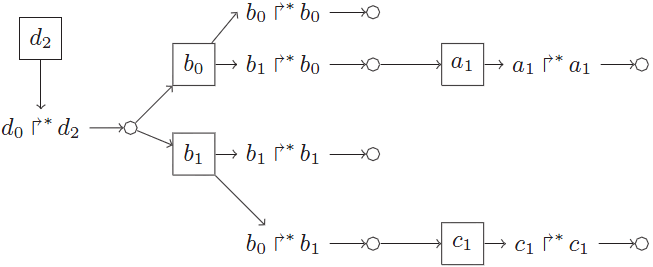
\includegraphics[scale=0.6]{underapp.png}
\caption{La structure abstraite $\lceil\mathcal{B}^\omega_\varsigma\rceil$ de l'exemple de Process Hitting dans le Figure \ref{phex} avec $\omega=d_0\Rsh^*d_2$ et $\varsigma=\langle a_1,b_1,c_1,d_0\rangle$, cet objectif est r\'ealisable.}
\end{figure}
\section{Cut set}
Le cut set une approche contraire \`a la compl\'etion, qui sert \`a emp\^echer d\'efinitivement l'accessibilit\'e de certain processus. Cette m\'ethode calcule les cut sets directement d'une structure abstraite d\'eriv\'ee du mod\`ele, qui rend l'analyse des grands r\'eseaux traitables \citep{Pauleve2013}.

\subsection*{D\'efinition pr\'eliminaires}
Supposons un GLC solide global $\mathcal{A}^\omega_\varsigma=(V^\omega_\varsigma,E^\omega_\varsigma)$, avec les accesseurs habituels pour les relations directes de n\oe uds : 
\begin{flalign*}
\mathsf{children}&:V^\omega_\varsigma\mapsto \mathcal{P}(V^\omega_\varsigma) & \mathsf{parents}&:V^\omega_\varsigma\mapsto \mathcal{P}(V^\omega_\varsigma)\\
\mathsf{children}(n)\triangleq&\{m\in V^\omega_\varsigma \mid (n,m)\in E^\omega_\varsigma\} & \mathsf{parents}(n)\triangleq&\{m\in V^\omega_\varsigma \mid (m,n)\in E^\omega_\varsigma\}\\
\end{flalign*}
En partant d'une valuation $\mathbb{V}$, nous associons chaque n\oe ud \`a un ensemble de cut N-ensemble, l'ensemble des cut N-ensembles peut \^etre raffin\'e par $\mathsf{update}(\mathbb{V},n)$:
\begin{itemize}
\item si $n$ est une solution $\langle P,ls\rangle\in \mathbf{Sol}$, il est suffisant d'emp\^echer l'accessibilit\'e de tout \'etat local $ls$; par cons\'equent, le cut N-ensemble est issu de l'union des ensembles des $\mathsf{children}$ de $n$.
\item si $n$ est un objectif $P\in\mathbf{Obj}$, tous ses solutions (dans $\mathsf{P}$) doivent \^etre enlev\'ees afin que $P$ ne soit pas r\'ealisable : alors les cut N-ensembles sont issus des cut N-ensembles des $\mathsf{children}$.
\item si $n$ est un \'etat local $a_i$, il est suffisant d'emp\^echer tous ses $\mathsf{children}$(objectifs) pour emp\^echer l'accessibilit\'e de $a_i$ \`a partir de tout \'etat dans le contexte $\varsigma$. Au fait, si $a_i\in\mathcal{O}$, $\{a_i\}$ sera rajout\'e dans l'ensemble de ses cut N-ensembles.
\end{itemize}
\begin{Def}[Valuation $\mathbb{V}$]
Une valuation $\mathbb{V}$ : $V^\omega_\varsigma\mapsto\mathcal{P}(\mathcal{P}^{\leq N}(\mathcal{O}))$ est un mappage de chaque n\oe ud de $\mathcal{A}^\omega_\varsigma$ \`a un ensemble de N-ensemble d'\'etats locaux. $\mathbf{Val}$ est l'ensemble de toutes les valuations. $\mathbb{V}_0\in\mathbf{Val}$ se r\'ef\`ere \`a la valuation telle que $\forall n \in V^\omega_\varsigma, \mathbb{V}_0(n)=\varnothing$.
\end{Def}
\begin{Def}[$\mathsf{update}$ : $\mathbf{Val}\times V^\omega_\varsigma\mapsto\mathbf{Val}$]
$$\mathsf{update}(\mathbb{V},n)\triangleq 
\begin{cases}
\mathbb{V}\{n\mapsto\zeta^N(\bigcup_{m\in \mathsf{children(n)}}\mathbb{V}(m))\}&\text{si }n\in\mathbf{Sol}\\
            \mathbb{V}\{n\mapsto\zeta^N({\prod_{m\in \mathsf{children(n)}}}\mathbb{V}(m))\}&\text{si }n\in\mathbf{Obj}\\
            \mathbb{V}\{n\mapsto\zeta^N({\prod_{m\in \mathsf{children(n)}}}\mathbb{V}(m))\}&\text{si }n\in\mathbf{LS}\setminus\mathcal{O}\\
            \mathbb{V}\{n\mapsto\zeta^N(\{\{a\}\}\cup{\prod_{m\in \mathsf{children(n)}}}\mathbb{V}(m))\}&\text{si }n\in\mathbf{LS}\cap\mathcal{O}
\end{cases}
$$
avec $\zeta^N(\{e_1,\ldots,e_n\})\triangleq\{e_i\mid i\in[1;n]\land\#e_i\leq N\land\nexists j\in[1;n],j\neq i,e_j\subset e_i\}$ o\`u $e_i$ sont des ensembles, et $\forall i\in[1;n]$.
\end{Def}
\`A partir de $\mathbb{V}_0$, nous pouvons appliquer \`a maintes reprises $\mathsf{update}$ pour tout n\oe ud de $\mathcal{A}^\omega_\varsigma$ pour raffiner sa valuation. Seuls les n\oe uds o\`u l'un de leurs $\mathsf{children}$ ont chang\'e de valeur
doivent \^etre prise en compte pour $\mathsf{update}$.

\'Etant donn\'e un ensemble d'\'etats locaux $\mathcal{O}\subseteq\mathbf{LS}$, cette section d\'edie \`a un algorithme du calcul de l'ensemble $\mathbb{V}(a_i)$  \`a partir de $\mathcal{A}^\omega_\varsigma$.\\
\begin{algorithm}[ht]\label{algocut}
$\mathcal{M}\gets V^\omega_\varsigma$\\
$\mathbb{V}\gets\mathbb{V}_0$\\
\While{$\mathcal{M}\neq\varnothing$}{$n\gets\text{argmin}_{m\in\mathcal{M}}\{\mathsf{rang}(m)\}$\\
		$\mathcal{M}\gets\mathcal{M}\setminus\{n\}$\\
		$\mathbb{V}'\gets\mathsf{update}(\mathbb{V},n)$\\
		\If{$\mathbb{V}'(n)\neq\mathbb{V}(n)$}{$\mathcal{M}\gets\mathcal{M}\cup\mathsf{parents}(n)$}
		$\mathbb{V}\gets\mathbb{V}'$}
\Return{$\mathbb{V}$} 
\end{algorithm}
o\`u $\mathsf{rank}(n)$ se r\'ef\`ere au rang topologique de $n$.

Une fois le GLC est \'etabli, il est possible de calculer le cut set, de complexit\'e moins importante que le parcours global. Sous l'aspect des actions, il est suffisant d'emp\^echer certain processus en enlevant les actions li\'ees d'un des cut sets.

Exemple:

\begin{figure}[ht]
\centering
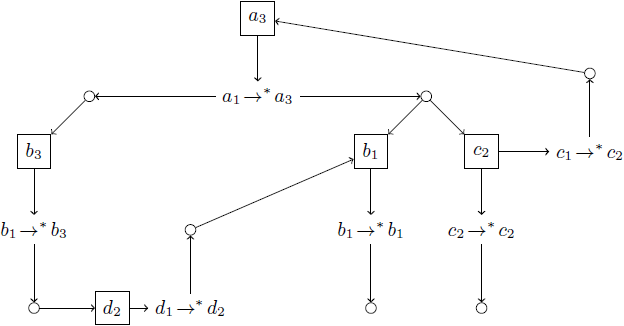
\includegraphics[scale=0.6]{cutset.png}
\caption{Exemple d'un GLC avec son objectif $a_1\to^*a_3$}
\end{figure}\label{figcut}
\begin{table}[ht]
\centering
\begin{tabular}{|c|c|l|}
 \hline 
 N\oe ud & $\mathsf{rang}$ & $\mathbb{V}$ \\ 
 \hline 
 $\langle b_1\to^*b_1,\varnothing\rangle$ & 1 & $\varnothing$ \\ 
 \hline 
 $b_1\to^*b_1$ & 2 & $\varnothing$ \\ 
 \hline 
 $b_1$ & 3 & $\{\{b_1\}\}$ \\ 
 \hline 
 $\langle d_1\to^*d_2,\{b_1\}\rangle$ & 4 & $\{\{b_1\}\}$ \\ 
 \hline 
 $d_1\to^*d_2$ & 5 & $\{\{b_1\}\}$ \\ 
 \hline 
 $d_2$ & 6 & $\{\{b_1\},\{d_2\}\}$ \\ 
 \hline 
 $\langle b_1\to^*b_3,\{d_2\}\rangle$ & 7 & $\{\{b_1\},\{d_2\}\}$ \\ 
 \hline 
 $b_1\to^*b_3$ & 8 & $\{\{b_1\},\{d_2\}\}$ \\ 
 \hline 
 $b_3$ & 9 & $\{\{b_1\},\{b_3\},\{d_2\}\}$ \\ 
 \hline 
 $\langle a_1\to^*a_3,\{b_3\}\rangle$ & 10 & $\{\{b_1\},\{b_3\},\{d_2\}\}$ \\ 
 \hline 
 $\langle c_2\to^*c_2,\varnothing\rangle$ & 11 & $\varnothing$ \\ 
 \hline 
 $c_2\to^*c_2$ & 12 & $\varnothing$ \\ 
 \hline 
 $c_2$ & 13 & $\{\{c_2\}\}$ \\ 
 \hline 
 $\langle a_1\to^*a_3,\{b_1,c_2\}\rangle$ & 13 & $\{\{b_1\},\{c_2\}\}$ \\ 
 \hline 
 $a_1\to^*a_3$ & 13 & $\{\{b_1\},\{b_3,c_2\},\{c_2,d_2\}\}$ \\ 
 \hline 
 $a_3$ & 13 & $\{\{a_3\},\{b_1\},\{b_3,c_2\},\{c_2,d_2\}\}$ \\ 
 \hline 
 $\langle c_2\to^*c_2,\{a_3\}\rangle$ & 13 & $\{\{a_3\},\{b_1\},\{b_3,c_2\},\{c_2,d_2\}\}$ \\ 
 \hline 
 \end{tabular}
 \caption{R\'esultat de l'ex\'ecution de l'Algorithme \ref{algocut} sur le GLC du Figure \ref{figcut}, dans la colonne de $\mathbb{V}$, il est suffisant d'emp\^echer un des ensemble de processus pour rendre certain objectif non-r\'ealisable, e.g.$\{\{a_3\},\{b_1\},\{b_3,c_2\},\{c_2,d_2\}\}$ veut dire r\'ealisabilit\'e de $(a_1\to^*a_3)=\lnot(a_3\lor b_1\lor(b_3\land c_2)\lor(c_2\land d_2))$}  
\end{table}
\chapter{Pr\'eparation avant compl\'etion}
Avant de nous engager la compl\'etion, il est important de pr\'eciser quelle partie \`a compl\'eter : les diff\'erences entre l'observation et la simulation. Voici les deux cas possibles,
\begin{enumerate}
\item l'absence de certain processus dans l'observation et la pr\'esence de ce processus dans la simulation\label{ob1}
\item la pr\'esence de certain processus dans l'observation et l'absence de ce processus dans la simulation\label{ob2}
\end{enumerate}
Dans le cas \ref{ob1}, il existe des actions en trop dans le mod\`ele, nous pouvons appliquer le cut set afin de trouver les actions erron\'ees. Dans le cas \ref{ob2}, il manque quelques actions. Pour les rajouter, les d\'emarches seront pr\'esent\'ees dans le chapitre \ref{complet} Compl\'etion. 

Quant \`a l'accessibilit\'e, on tient compte de 2 aspects : l'efficacit\'e et l'exactitude, mais ces 2 aspects se contredisent souvent l'un l'autre. Dans la section suivante, deux m\'ethodes seront pr\'esent\'ees.
\section{M\'ethode non-exhaustive}
\`A l'aide de la commande \texttt{ph-reach} de {\Large P}INT (Analyse de sur-approximation et sous-approximation), on a 3 valeurs possibles de l'accessibilit\'e : non-accessible (non pour sur-approximation), inconclusive (oui pour sur-approximation et non pour sous-approximation, ce qui nous ne m\`ene pas \`a un r\'esultat d\'efinitif), accessible (oui pour sous-approximation). En fait, il arrive rarement que les r\'esultats soient inconclusifs, c'est-\`a-dire nous pouvons d\'eterminer dans la plupart de cas l'accessibilit\'e de certain processus \citep{Pauleve2012}.
\begin{table}[ht]
\centering
\begin{tabular}{|c|c|c|}
\hline
Sur-approximation & Sous-approximation & Accessibilit\'e\\
\hline
vrai & vrai & vrai\\
\hline
vrai & faux & inconclusive\\
\hline
faux & vrai & N/A\\
\hline
faux & faux & faux\\
\hline
\end{tabular}
\caption{Table de v\'erit\'e de l'accessibilit\'e}\label{tab2}
\end{table}

\section{M\'ethode exhaustive}
Nous fournissons \'egalement une autre approche en cas d'inconclusivit\'e et elle est capable d'analyser non seulement l'accessibilit\'e d'un processus mais la r\'ealisabilit\'e d'une s\'equence stricte. Cette approche est de parcourir toutes les branches de transitions de Process Hitting qui donne d\'efinitivement l'accessibilit\'e, mais avec une complexit\'e importante th\'eorique. Intuitivement, gr\^ace aux nombreux conditions de sortir, la complexit\'e dans la plupart de cas deviendrait moins importante.
\subsection{D\'efinitions Pr\'eliminaires}
\begin{Def}[Observabilit\'e]
Une sorte est consid\'er\'ee observable si ses donn\'ees temporis\'ees sont disponibles pendant l'exp\'erience, et toutes les sortes sont attribu\'ees inobservable par d\'efaut.
\end{Def}
\begin{Def}[S\'equence]
Une s\'equence est compos\'ee de processus dans l'ordre d'occurrence. Une s\'equence est dite r\'ealisable s'il y a un sc\'enario dans lequel les processus sont de m\^eme ordre d'occurrence que la s\'equence.
\end{Def}
\begin{Def}[S\'equence stricte]
Une s\'equence est stricte si elle contient toutes les \'evaluations des sortes observables, et les sortes inobservables ne doivent pas \^etre dans une s\'equence stricte.
\end{Def}
\begin{Def}[Ensemble d'actions valables]
Cet ensemble d\'esigne toutes les actions tirables dans l'\'etat actuel, not\'e $A=\{\acm{a_i}{b_j}{b_k}\mid s[a]=a_i\land s[b]=b_j\}$
\end{Def}
\begin{Def}[Op\'erateur override $\Cap$ : $\mathbf{Ctx\times\mathcal{P}(Proc)\mapsto Ctx}$]
\'Etant donn\'e un contexte $\varsigma\in\mathbf{Ctx}$ et $ps\in\mathcal{P}(\mathbf{Proc})$, l'override de $\varsigma$ par $ps$ est not\'e $\varsigma\Cap ps$ :
\begin{equation}
\forall a \in\Sigma,(\varsigma\Cap ps)[a]\triangleq
\left\{
\begin{aligned}
&\{p\in ps\mid \Sigma(p)=a\}&&si\ \exists p\in ps,\Sigma(p)=a\\
&\varsigma[a]&&sinon
\end{aligned}
\right.
\nonumber
\end{equation} 
Exemple de l'op\'erateur $\Cap$ : $\langle a_1,a_2,b_1,c_1\rangle\Cap\{a_3,b_2,b_3\}=\langle a_3,b_2,b_3,c_1\rangle$.
\end{Def}
\begin{figure}[ht]
\centering
\begin{tikzpicture}%[font=\scriptsize]
%\path[use as bounding box] (0,-1) rectangle (4,4);

\TSort{(0,0)}{a}{2}{l}
\TSort{(4,0)}{b}{2}{r}
\THit{a_0}{out=0,in=210}{b_1}{.west}{b_0}
\THit{a_1}{out=60,in=30}{b_0}{.east}{b_1}
\THit{b_0}{out=210,in=210}{a_0}{.west}{a_1}
\THit{b_1}{out=170,in=0}{a_1}{.east}{a_0}

\path[bounce,bend right]
\TBounce{b_1}{}{b_0}{.west}
\TBounce{b_0}{}{b_1}{.east}
;
\path[bounce,bend left]
\TBounce{a_1}{}{a_0}{.east}
;
\path[bounce,bend left]
\TBounce{a_0}{}{a_1}{.west}
;
\TState{a_0,b_0}
\end{tikzpicture}
\caption{Exemple de s\'equence stricte:
Il y a 4 actions: $\mathscr{H}=\{a_0\to b_1\Rsh b_0$, $a_1\to b_0\Rsh b_1$, $b_0\to a_0\Rsh a_1$, $b_1\to a_1\Rsh a_0\}$, avec l'\'etat initial $\varsigma=\langle a_0, b_0\rangle$, supposons les sortes $a$ et $b$ sont observables, la sequence $S_1=a_1:\,:b_1$ est stricte alor que la sequence $S_2=b_1$ n'est pas stricte, comme le seul sc\'enario est $\delta=b_0\to a_0\Rsh a_1:\,:a_1\to b_0\Rsh b_1...$
}
\end{figure}
\subsection{Description du probl\`eme}
\'Etant donn\'e un Process Hitting $PH=(\Sigma, L, \mathscr{H})$, un contexte $\varsigma$ (On tient compte des \'etats initiaux de toutes les sortes (y compris ceux des sortes inobservables)), une s\'equence stricte probablement non r\'ealisable pour l'instant : $S=p_1:\,:p_2:\,:\ldots:\,:p_{|S|}$, nous voulons classer le(les) processus inaccessible(s) pour la prochaine d\'emarche (la compl\'etion).
\subsection{Dynamique}
Pour noter l'\'evolution de mod\`ele, $s_0=\varsigma$, $s_i=s_{i-1}\Cap\ p_i$, o\`u $i$ est l'indexe des \'etapes et les $s_i$ sont les \'etats globaux et les $p_i$ sont les processus chang\'es apr\`es transitions et $A_i$ les actions valables \`a l'\'etape $i$.

\begin{itemize}
\item Si $Card(A_i) = 0$, il n'y a aucune action valable, le syst\`eme atteint un \'etat stable;
\item Si $Card(A_i) = 1$, il n'y a qu'une seule action valable, le syst\`eme va dans un seul sens;
\item Si $Card(A_i) > 1$, il y a des branches dans l'\'evolution, et les overrides possibles du prochain instant seront enregistr\'es dans \texttt{futureActions}.

O\`u $Card(A)$ signifie le cardinal de l'ensemble $A$.
\end{itemize}

\subsection{Classification des cas}\label{class}
Chaque fois apr\`es tirer une action (transition), l'analyse du premier processus dans la s\'equence stricte $S$ est faite comme suit:
\begin{enumerate}[label=\arabic*,align=left]
	\item Processus inaccessible (processus sans actions li\'ees): retourner 1 dans \texttt{realisablility} puis ajouter ce processus dans \texttt{unreachableProcess1};\label{12}
	\item Processus inaccessible (processus avec actions li\'ees mais il n'y a aucune action valable ou l'\'etat actuel est pareil que celui qui est apparu avant (boucle)): retourner 1 dans \texttt{realisablility} puis ajouter ce processus dans \texttt{unreachableProcess2};\label{13}
	\item Accessible mais dans mauvais ordre : retourner 2 dans \texttt{realisablility}, puis ajouter ce processus dans \texttt{unreachableProcess2}, il y a alors 2 cas de mauvais ordre :\label{14}
	\begin{enumerate}[label=\Roman*,align=left]\label{15}
		\item Un dernier processus dans la s\'equence appara\^it plus t\^ot que ceux des anciens;
		\item Un processus observable appara\^it mais il n'est pas dans la s\'equence.
	\end{enumerate}
	\item Processus accessible : enlever ce processus dans la s\'equence; lorsque la s\'equence devient vide, retourner 0 dans \texttt{realisablility} (cette s\'equence est bien r\'ealisable);\label{16}
	\item S'il y a des branches dans la transition, on consid\`ere : 
	\begin{enumerate}[label=\Roman*,align=left]
		\item Ce processus est accessible s'il est accessible depuis au moins une des branches. (Class\'e dans le cas \ref{16});
		\item Il n'y a aucune branche valable pour que ce processus soit accessible :
		\begin{enumerate}[label=\roman*,align=left]
			\item Toutes ses branches m\`enent au cas \ref{14}, retourner 2 dans \texttt{realisablility}
			\item Il y a au moins une branche qui m\`ene au cas \ref{12} ou \ref{13}, retourner 1 dans \texttt{realisablility}
		\end{enumerate}
	\end{enumerate}
\end{enumerate}
Dans la classification, il y a 3 valeurs de retour possibles, 0 indique la r\'ealisabilit\'e de la s\'equence, 1 indique que la s\'equence n'est pas r\'ealisable \`a cause de l'inatteignabilit\'e de certain processus, 2 indique que la s\'equence n'est pas r\'ealisable non plus, mais \`a cause du mauvais ordre d'apparition.

Exemple de mauvais ordre : la s\'equence dans l'observation est $S_o=p_1:\,:p_2:\,:p_3$, mais selon la simulation, nous n'avons que $S_s=p_2:\,:p_1:\,:p_3$ comme r\'esultat. Bien que les processus soient accessible, ils n'apparaissent pas dans un bon ordre.

Comme expliqu\'e avant, cette approche peut \^etre appliqu\'ee en cas d'inconclusivit\'e de la m\'ethode non-exhaustive. En prenant la s\'equence stricte avec un seul processus,  
L'Algorithme \ref{a2} r\'ealise cette id\'ee, bien que la complexit\'e est importante, la s\'equence stricte la r\'eduit efficacement en utilisant les donn\'ees temporis\'ees\footnote{Le code est disponible sur https://github.com/XinweiChai/Completion/tree/master/src/completion}.
\chapter{Compl\'etion}\label{complet}
\section{Motivation}
L'analyse des r\'eseaux de r\'egulation, qui comprend les r\'eseaux g\'en\'etiques, les r\'eseaux d'interaction entre les prot\'eines et les r\'eseaux de signaux, est donc un des th\`emes principaux en bioinformatique.

Le but est souvent : avec les informations d'expression d'une s\'erie de g\`enes (une s\'erie d'\'etats de tous les g\`enes dans un environnement vari\'e), on peut en d\'eduire les fonctions avec des g\`enes d'entr\'ee qui r\'egule chaque g\`ene, avec lesquelles un r\'eseau g\'en\'etique est form\'e, mais dans le cas d'un r\'eseau de r\'egulation, il existe toujours des donn\'ees inconnues (niveaux d'activation et les relations entre des n\oe uds) pour certains g\`enes, prot\'eines, etc, et qu'il existe aussi des donn\'ee erron\'ees \citep{Akutsu2009}. Il est indispensable de chercher les m\'ethodes pour compl\'eter les r\'eseaux et pour les modifier avec afin d'avoir la dynamique compl\`ete du syst\`eme. Souvent, la compl\'etion est assez importante. Dans cet article, trois m\'ethodes de compl\'etion seront pr\'esent\'ees, dont l'une est \`a l'aide d'un seul processus, et les deux sont \`a partir d'une s\'equence de processus.

Si on dit le cut set ``coupe'' la possibilit\'e d'atteindre certain \'etat local, alors la compl\'etion est l'op\'eration inverse de cut set, car elle donne la possibilit\'e d'acc\'eder les processus inatteignable, mais elle donne souvent de nouvelles branches qui ne sont pas issus du syst\`eme original.

\begin{figure}
\centering
\begin{tikzpicture}
\node at (0,0)[anchor=east] {\small accessible2};
\node at (0,1)[anchor=east] {\small accessible1};
\node at (0,-1)[anchor=east] {\small inconclusif1};
\node at (1.4,0)[anchor=west] {\small inaccessible};
\draw[<->] (0,0) -- (1.4,0);
\draw[<->] (0,1) -- (1.4,0.1);
\draw[<->] (0,-1) -- (1.4,-0.1);
\end{tikzpicture}
\caption{La surjection de cas accessible au cas inaccessible (cutset $\leftrightarrows$ compl\'etion)}\label{surj}
\end{figure}
Exemple :

Prenons l'exemple de Figure \ref{phex}, supposons $\varsigma=\langle a_0,b_0,c_0,d_1\rangle$ et 
$$\mathscr{H}=\{\acm{a_0}{c_0}{c_1},\acm{a_1}{b_1}{b_0},\acm{c_1}{b_0}{b_1},$$
$$\acm{b_1}{a_0}{a_1},\acm{b_0}{d_0}{d_1},\acm{d_1}{b_0}{b_2},\acm{c_1}{d_1}{d_0}\}$$
avec \ac{b_2}{d_0}{d_2} et \ac{b_1}{d_1}{d_2} relev\'ees, maintenant $d_2$ n'est pas accessible. Pour que $d_2$ soit accessible, il y a une alternative entre ces deux actions, mais il n'y a pas d'informations en plus pour d\'eterminer.

\begin{figure}[ht]
\centering
\begin{tikzpicture}%[font=\scriptsize]
%\path[use as bounding box] (0,-1) rectangle (4,4);
%{left, right, top, bottom}
\TSort{(0,0)}{a}{2}{l}
\TSort{(4,0)}{b}{3}{l}
\TSort{(8,0)}{d}{3}{r}
\TSort{(3,-2)}{c}{2}{b}
\THit{a_1}{}{b_1}{.west}{b_0}
\THit{a_0}{}{c_0}{.north}{c_1}
\THit{b_1}{}{a_0}{.east}{a_1}
\THit{c_1}{out=120,in=255}{b_0}{.west}{b_1}
\THit{b_0}{}{d_0}{.west}{d_1}
\THit{b_1}{color=red}{d_1}{.west}{d_2}
\THit{b_2}{bend right=45,in=-30,color=red}{d_0}{.east}{d_2}
\THit{d_1}{}{b_0}{.north east}{b_2}
\THit{c_1}{bend right=150,out=-90,in=-90}{d_1}{.south east}{d_0}

\path[bounce,bend right]
\TBounce{b_1}{}{b_0}{.north}
\TBounce{a_0}{}{a_1}{.south}
\TBounce{d_0}{}{d_2}{.south}
\TBounce{b_0}{}{b_2}{.south}
;
\path[bounce,bend left]
\TBounce{d_0}{}{d_1}{.south}
\TBounce{b_0}{}{b_1}{.south}
\TBounce{c_0}{}{c_1}{.west}
\TBounce{d_1}{}{d_2}{.south}
\TBounce{d_1}{}{d_0}{.north}
;
\path[bounce,bend left]
;
\TState{a_0,b_1,c_0,d_0}
\end{tikzpicture}
\caption{Compl\'etion du Process Hitting en rajoutant l'action \ac{b_2}{d_0}{d_2} ou \ac{b_1}{d_1}{d_2}}
\end{figure}
\`A cause de cette surjectivit\'e, le choix d\'efinitif exige plus d'exp\'eriences et d'analyses.(Dans cet exemple, l'analyse sur $b_1,b_2$ ou $c_1$ est possible)

Les r\'esultats de compl\'etion diff\`erent \`a cause de l'approche de d\'etermination de l'accessibilit\'e de processus (ou bien la r\'ealisabilit\'e de s\'equence stricte).

\begin{itemize}
\item En utilisant {\Large P}INT : non-accessible $\to$ non conclusive/accessible
\item En utilisant la m\'ethode exhaustive : non-accessible $\to$ accessible
\end{itemize} 
Par la suite, nous proposons deux m\'ethodes de compl\'etion d'un r\'eseau Process Hitting, qui servent \`a ces deux cas.
\section{D\'efinitions pr\'eliminaires}
Comme il y a des donn\'ees inconnues dans le r\'eseau de r\'egulation, on fait des hypoth\`eses sur les relations de r\'egulation et les v\'erifie si elles sont coh\'erentes avec l'exp\'erience.
\begin{Def}[Relation de r\'egulation] L'activation ou l'inhibition de la sorte $a$ sur la sorte $b$ est not\'ee $r=(a,b,\alpha_{ab})$, l'ensemble de toutes les relations de r\'egulation est d\'efini comme :
$R=\{(a,b,\alpha_{ab})\mid  (a,b)\in\Sigma^2\land \alpha_{ab}\in\{+,-\} \}$.
\end{Def}
\begin{Def}[Coh\'erence]
Une action $a=\acm{a_i}{b_j}{b_k}$ est dite \textit{incoh\'erente} avec $R$ si 
\begin{align*}
\exists r\in R,&(r=(a,b,+)\land ((i=l_a\land j>k)\lor(i=0\land j<k)))\lor\\
&(r=(a,b,-)\land ((i=l_a\land j<k)\lor(i=0\land j>k)))
\end{align*}
sinon, elle est consid\'er\'ee coh\'erente avec $R$.
\end{Def}
Exemple :

Le Figure \ref{figres} (a), si les relations de r\'egulation entre $u$ et $v$ restent \`a v\'erifier, c'est-\`a-dire $R=\{(u,v,+),(v,u,-),(u,u,+)\}$, et si on prend un formalisme de Process Hitting, l'action \ac{v_1}{u_1}{u_2} n'est pas coh\'erente avec $R$.
\section{Compl\'etion bas\'e sur la s\'equence stricte}\label{1}
\subsection*{Description du probl\`eme}
\'Etant donn\'e un Process Hitting $PH$, un ensemble de relations de r\'egulation $R$ et une s\'equence stricte $S$, il est suffisant d'analyser la r\'ealisabilit\'e de $S$ en utilisant la m\'ethode exhaustive. Au d\'ebut, la s\'equence observ\'ee est souvent irr\'ealisable pour le r\'eseau original, nous voulons le compl\'eter en rajoutant des actions pour que le mod\`ele ait les m\^emes comportements.

L'id\'ee est : dans la s\'equence stricte $S=p_1:\,:\ldots p_n$, supposons que apr\`es l'analyse de r\'ealisabilit\'e, le premier processus inaccessible $p_i$ avec $1\le i\le n$ a \'et\'e trouv\'e. Ensuite, appliquer la compl\'etion (rajouter des actions) pour que $p_i$ soit accessible. Puis reprendre l'analyse de r\'ealisabilit\'e de $S$, un autre processus inaccessible $p_j$ avec $i\le j\le n$ est trouv\'e. Refaire les d\'emarches avant, jusqu'\`a ce que la s\'equence est r\'ealisable.

Voici l'algorithme r\'ep\'etitif qui r\'ealise cette id\'ee.

\begin{algorithm}[ht]
 \KwData{Un fichier \texttt{.ph} en ajoutant une s\'equence stricte \texttt{sequence} et un ensemble de relations de r\'egulation \texttt{relation}}
 \KwResult{Un Process Hitting compl\'et\'e}
 \Repeat {\texttt{Realisability}=0}{
 Algorithme \ref{a1} Transition\\
 Algorithme \ref{a2} Realisability\\
 Algorithme \ref{a3} Classification\\
 Algorithme \ref{a4} {\bf ou} Algorithme \ref{a5} Compl\'etion selon \texttt{relation}}
 \caption{Structure de programme (Algorithmes mentionn\'es sont dans l'annexe)}
\end{algorithm}
Nous aimerons d\'etailler l'id\'ee de Algorithme \ref{a4} et Algorithme \ref{a5}, la compl\'etion : apr\`es avoir appliqu\'e la m\'ethode exhaustive et la classification des processus inaccessibles, on a plusieurs valeurs de retour possibles, l'id\'ee de compl\'etion est comme suit\footnote{Le code est disponible sur https://github.com/XinweiChai/Completion/tree/master/src/completion}, 

Si la valeur de retour (dans la section \ref{class}) est :
\begin{enumerate}\setcounter{enumi}{-1}
	\item la s\'equence est bien r\'ealisable, pas de n\'ecessit\'e de faire la compl\'etion;
	\item  diff\'erent types de inaccessibilit\'e de processus :\label{cas1}
	\begin{enumerate}[label=\Roman*,align=left]
		\item \texttt{unreachableProcess1}: supposons $a_j$ est un (ou le seul) de ses \'el\'ement(s), ajouter action : 				$b_k\rightarrow a_j\Rsh a_i$ s'il y a une relation de r\'egulation de forme $(b,a,\pm)$ dans $R$;		
		\item \texttt{unreachableProcess2}: supposons $a_j$ est un (ou le seul) de ses \'el\'ement(s), et $b_k\rightarrow a_j\Rsh a_i$ est une de ses actions li\'ees, v\'erifier si $a_j$ et $b_k$ sont dans les \'etats actuels:
		\begin{enumerate}[label=\roman*,align=left]
			\item si oui, il est s\^ur que $b_k$ n'est pas accessible, sinon $a_i$ sera accessible. Classer $b_k$ (dans la  Section \ref{class}) et refaire le traitement que l'on a fais \`a $a_i$ \ldots c'est une t\^ache r\'ecursive sans garantie de terminaison \`a cause de la boucle\footnote{par exemple les actions \ac{b_k}{a_j}{a_i} et \ac{a_i}{b_m}{b_k} forme une boucle, le raisonnement n'arr\^ete jamais}, par cons\'equent il est n\'ecessaire de noter tous les bounces li\'es \`a ce calcul, si on trouve la r\'ep\'etition de certain bounce, alors l'action li\'ee (\ac{b_k}{a_j}{a_i} dans ce cas-l\`a) sera enlev\'ee de $\mathbf{LA}$;
			\item si $b_k$ est accessible, alors $a_i$ n'est pas accessible, traiter de m\^eme fa\c con comme \ref{2};
			\item si ni $a_i$ ni $b_k$ n'est accessible, enlever $b_k\rightarrow a_j\Rsh a_i$ des actions li\'ees de $a_i$, puis:
			\begin{description}
				\item[\quad] s'il y a d'autres actions li\'ees, essayer la compl\'etion avec une prochaine action;
				\item[\quad] s'il n'y a pas d'autres action li\'ees, ajouter $a_j$ \`a \texttt{unreachableProcess1} et enlever $a_j$ de \texttt{unreachableProcess2}.
			\end{description}
		\end{enumerate}
	\end{enumerate}
\item il y a peut-\^etre des erreurs dans le r\'eseau original, mais on peut quand m\^eme compl\'eter ce r\'eseau comme dans le cas \ref{cas1};
\end{enumerate}

Exemple : 
Un Process Hitting $PH=(\Sigma,L,\mathscr{H})$ avec $\Sigma=\{a,b\}$, $L=\{a_0,a_1\}\times\{b_0,b_1\}$, $\mathscr{H}=\{\acm{b_0}{a_0}{a_1},\acm{a_1}{b_0}{b_1}\}$, son contexte $\varsigma=\{a_0,b_0\}$, l'ensemble de relations de r\'egulation $R=\{(a,b,+),(b,a,-)\}$, et une s\'equence stricte $S=a_1:\,:b_1:\,:a_0:\,:b_0$.

\begin{figure}[ht]
\centering
\begin{tikzpicture}
\TSort{(0,0)}{a}{2}{l}
\TSort{(3,0)}{b}{2}{r}
\THit{a_1}{}{b_0}{.west}{b_1}
\THit{b_0}{}{a_0}{.east}{a_1}
\path[bounce,bend right]
\TBounce{a_0}{}{a_1}{.south east}
;
\path[bounce,bend left]
\TBounce{b_0}{}{b_1}{.west}
;
\TState{a_0,b_0}
\end{tikzpicture}
\qquad
\begin{tikzpicture}
\coordinate (P1) at (0,0);
\coordinate (P2) at (1,0);
\coordinate (P3) at (1,-1.5);
\coordinate (P4) at (0,-1.5);
\node at (P1)[anchor=east]{$(a_0,b_0)$};
\node at (P2)[anchor=west]{$(a_1,b_0)$};
\node at (P3)[anchor=west]{$(a_1,b_1)$};
\node at (P4)[anchor=east]{$(a_0,b_1)$};
\draw[->](P1)--(P2);
\draw[<-](-0.6,-0.25)--(-0.6,-1.25);
\draw[->](P3)--(P4);
\draw[->](1.6,-0.25)--(1.6,-1.25);
\end{tikzpicture}
\caption{Process Hitting original et son graphe de transition d\'eduit par la s\'equence strict}
\end{figure}
D'abord, $S'=a_1:\,:b_1$ est bien r\'ealisable, mais $a_0$ n'est pas accessible dans l'\'etat $\{a_1,b_1\}$, selon $(b,a,-)$, \ac{b_1}{a_1}{a_0} est ajout\'ee (coh\'erente). On relance la simulation et on trouve que pour l'instant, $a_0$ est accessible, mais $b_0$ n'est pas accessible dans l'\'etat $\{a_0,b_1\}$, on rajoute \ac{a_0}{b_1}{b_0} selon $(a,b,+)$, enfin, $S=a_1:\,:b_1:\,:a_0:\,:b_0$ est r\'ealisable apr\`es compl\'etion.

En plus, pour enregistrer les nouvelles donn\'ees, le fichier \texttt{.ph} est modifi\'e en rajoutant une s\'equence et des relations de r\'egulation. Les donn\'ees rajout\'ees sont sous la forme:
\vspace{0.2cm}
\hrule
\begin{verbatim}
sequence a 1 b 1 a 0 b 0
relation a b + b a -
\end{verbatim}
\hrule
\section{Compl\'etion bas\'ee sur le processus}
Compl\'etion bas\'ee sur le processus est un probl\`eme plus simple que celle avant, car un processus est une s\'equence contenant un seul \'el\'ement. L'int\'er\^et de cette section est de rendre la complexit\'e moins importante. Dans l'algorithme de Section \ref{1}, la partie Algorithme \ref{a1} est exhaustive, qui parcourt toutes les branches pour v\'erifier leur accessibilit\'e. Le probl\`eme de compl\'etion sera peut-\^etre intraitable \`a grande \'echelle.

Pour analyser l'accessibilit\'e d'un certain processus, \texttt{ph-reach} peut remplacer l'Algorithme \ref{a1}, et on fais aussi la classification des processus inaccessibles et la partie de compl\'etion ressemble \`a Section \ref{1}, sauf il n'y a pas de possibilit\'e de la valeur de retour 2 dans le cas de la compl\'etion bas\'ee sur la s\'equence stricte.

Supposons $a_i$ est le processus inaccessible.\footnote{Le code est disponible sur https://github.com/XinweiChai/Completion/tree/master/src/completion}
	\begin{enumerate}[label=\arabic*,align=left]
		\item \texttt{unreachableProcess1}: ajouter action $b_k\rightarrow a_j\Rsh a_i$ s'il existe une relation de r\'egulation de forme $(b,a,\pm)$ dans $R$;		
		\item \texttt{unreachableProcess2}: supposons $b_k\rightarrow a_j\Rsh a_i$ est une de ses actions li\'ees, v\'erifier si $a_j$ est accessible;
		\begin{enumerate}[label=\roman*,align=left]
			\item \label{2}si $a_j$ est accessible, il est s\^ur que $b_k$ n'est pas accessible, sinon $a_i$ sera accessible. Classer $b_k$ (dans la Section \ref{cas1}) et refaire le traitement que l'on a fais pour $a_i$, c'est une t\^ache r\'ecursive sans garantie de terminaison de m\^eme raisons que la section pr\'ec\'edente, par cons\'equent il est n\'ecessaire de noter tous les bounces li\'es \`a ce calcul, si on trouve la r\'ep\'etition de certain bounce, alors l'action li\'ee (\ac{b_k}{a_j}{a_i} dans ce cas-l\`a) sera enlev\'ee de $\mathbf{LA}$;
			\item si $b_k$ est accessible, traiter de m\^eme fa\c con comme \ref{2}
			\item si ni $a_j$ ni $b_k$ n'est accessible, enlever $b_k\rightarrow a_j\Rsh a_i$ des actions li\'ees de $a_i$, puis:
			\begin{description}
				\item[\quad] s'il y a d'autres actions li\'ees, essayer la compl\'etion avec une prochaine action;
				\item[\quad] s'il n'y a pas d'autres action li\'ees, ajouter $a_j$ \`a \texttt{unreachableProcess1} et supprimer $a_j$ de \texttt{unreachableProcess2}.
			\end{description}
		\end{enumerate}
	\end{enumerate}

L'algorithme global deviendra :

\begin{algorithm}[ht]
\KwData{Un fichier \texttt{.ph}, un processus inatteignable \texttt{p} et l'ensemble de relations de r\'egulation \texttt{relation}}
 \KwResult{Un Process Hitting compl\'et\'e}
 \Repeat {\texttt{ph-reach}= true {\bf ou} inconclusive}{
 Appliquer \texttt{ph-reach} sur \texttt{p}\\
 Algorithme \ref{a3} Classification\\
 Algorithme \ref{a4} {\bf ou} Algorithme \ref{a5} Compl\'etion selon \texttt{relation}}
 \caption{Structure de programme}
\end{algorithm}
En plus, cette m\'ethode peut \^etre encore simplifi\'ee en appliquant seulement la sur-approximation, comme l'accessibilit\'e cherch\'ee ne d\'epend pas de la sous-approximation (la logique indiqu\'e dans le tableau \ref{tab2}).

Exemple :\\
\'Etant donn\'e un Process Hitting $PH=(\Sigma,L,\mathscr{H})$ avec $\Sigma=\{a,b,c\}$, $L=\{a_0,a_1\}\times\{b_0,b_1\}\times\{c_0,c_1\}$, $\mathscr{H}=\{\acm{a_1}{b_0}{b_1}\}$, son contexte $\varsigma=\{a_0,b_0,c_0\}$, et la relation de r\'egulation $R=\{(a,b,+),(c,a,-)\}$.

\begin{figure}[ht]
\centering
\begin{tikzpicture}
\coordinate (P1) at (0,0);
\node at (P1) {{\Large c}};
\coordinate (P2) at (2,0);
\node at (P2) {{\Large a}};
\coordinate (P3) at (4,0);
\node at (P3) {{\Large b}};
\coordinate (P4) at ($(P2)+(150:0.6)$);
\draw (P1) circle(0.4) ;
\draw (P2) circle(0.4);
\draw (P3) circle(0.4);
\draw [line width=1pt](30:0.5) .. controls  (1,0.7) .. (P4);
\draw [->, line width=1pt]($(P2)+(30:0.5)$) .. controls  (3,0.7) .. ($(P3)+(150:0.55)$);
\draw [line width=1pt]($(P4)+(45:0.15)$) -- ($(P4)-(45:0.15)$);
\end{tikzpicture}\qquad
\begin{tikzpicture}%[font=\scriptsize]
%\path[use as bounding box] (0,-1) rectangle (4,4);

\TSort{(0,0)}{c}{2}{l}
\TSort{(3,0)}{a}{2}{r}
\TSort{(6,0)}{b}{2}{r}
\THit{a_1}{}{b_0}{.west}{b_1}
\THit{c_0}{color=red}{a_0}{.west}{a_1}


\path[bounce,bend left]
\TBounce{b_0}{}{b_1}{.west}
\TBounce{a_0}{}{a_1}{.west}
;
\TState{a_0,b_0,c_0}
\end{tikzpicture}
\caption{
Au d\'ebut, $b_1$ n'est pas accessible, comme il a une action li\'ee \ac{a_1}{b_0}{b_1}, $b_1$ est class\'e dans \texttt{unreachableProcess2}. $a_0$ est \'evidemment inaccessible car $b_0$ est accessible (\'etat initial). Selon $(c,a,-)\in R$, \ac{c_0}{a_0}{a_1} est rajout\'ee, alors $b_1$ devient accessible.
}
\end{figure}
Nous pouvons aussi simplifier le calcul de sur-approximation, comme dans l'article de Paulev\'e \textit{et al.} \citep{Pauleve2012}, la structure abstraite $\mathcal{A}^\omega_\varsigma$ est de forme $processus\to objectif\to solution \to processus \cdots$, mais il n'y a qu'un seul objectif suivi d'un processus. Alors le GLC peut \^etre ainsi simplifi\'e : $processus\to solution\to processus\cdots$.
\begin{figure}[ht]
\centering
\begin{tikzpicture}
\draw (0,0) rectangle (0.5,0.5);
\coordinate (P1) at (0.5,0.25);
\coordinate (P2) at ($(P1)+(1,0)$);
\draw [->](P1) -- (P2);
\coordinate (P3) at ($(P2)+(2pt,0)$);
\draw (P3) circle(2pt);
\node at ($(P3)+(0.6,0)$){and};
\coordinate (P4) at ($(P3)+(30:2pt)+(30:1)$);
\draw[->] ($(P3)+(2pt,0)$) -- (P4);
\draw (P4) rectangle ++(0.5,0.5);
\coordinate (P5) at ($(P3)+(-30:2pt)+(-30:1)$);
\draw[->] ($(P3)+(2pt,0)$) -- (P5);
\draw (P5) rectangle ++(0.5,-0.5);
\coordinate (P6) at ($(0.25,0)+(-60:1)$);
\draw [->](0.25,0) -- (P6);
\draw ($(P6)+(-60:2pt)$) circle(2pt);
\node at ($(P6)+(0,0.6)$){or};
\end{tikzpicture}
\caption{Le raisonnement local avec les n\oe uds dans la sur-approximation : les carr\'es repr\'esentent les processus , et les cercles repr\'esentent les solutions}
\end{figure}
\section{Compl\'etion bas\'ee sur le syst\`eme retard\'e}
Dans cette section, nous allons introduire une autre m\'ethode de compl\'etion de Process Hitting bas\'ee sur le syst\`eme retard\'e propos\'ee par Ben Abdallah \textit{et al.} \citep{Abdallah2014,Abdallah2015}. Cette approche fonctionne de fa\c con exhaustive mais limit\'ee, en prenant les donn\'ees d'observation de forme d'un chronogramme. Par le calcul de d\'elai de chaque action, on d\'ecide enfin les actions rajout\'ees. Ce probl\`eme est r\'esolue \`a l'aide de l'ASP \citep{Baral2003}, un langage tr\`es concis et efficace. 

\subsection{Syst\`eme biologique retard\'e}
\begin{Def}[Action plurielle temporis\'ee]
\'Etant donn\'e un Process Hitting $PH=(\Sigma,L,\mathcal{H})$. Une action plurielle est not\'ee : $h=A\stackrel{D}{\to}b_j\Rsh b_k$ avec $A\in \mathcal{L}^{\diamond}\land b_j\neq b_k\ \land$ si $\ b_i\in A\Rightarrow A=\{b_j\}$. O\`u $\mathcal{L}^{\diamond}$ est l'ensemble de tous les sous-ensembles de $\mathcal{L}$ et $D$ le d\'elai de l'action.
\end{Def}
Avec ces nouvelles actions, un syst\`eme retard\'e model\'e en Process Hitting peut \^etre construit. 
\begin{Def}[Process Hitting avec actions plurielles temporis\'ees]
\'Etant donn\'e un Process Hitting $PH=(\Sigma,L,\mathscr{H})$, en changeant $\mathscr{H}$ en $\mathscr{H}_{tp}=\{A\stackrel{D}{\to}b_j\Rsh b_k\mid A\in\mathcal{L}^{\diamond},b_j\neq b_k,b_i\in A\Rightarrow A=\{b_j\}\}$ qui est l'ensemble fini des actions plurielles temporis\'ees, le nouveau Process Hitting $PH=(\Sigma,L,\mathscr{H}_{tp})$ est appel\'e Process Hitting avec actions plurielles temporis\'ees.
\end{Def}
\subsection{Algorithme}

Cette approche (Algorithme \ref{sysret}) prend en compte toutes les possibilit\'es d'ajout d'actions du r\'eseau, mais \`a cause de la s\'emantique retard\'ee, il n'est pas possible de d\'ecider si une action rajout\'ee est correcte ou non. On consid\`ere que le r\'esultat avec le minimum de modifications tel que l'observation et le mod\`ele soient coh\'erents est le plus ``correct''. 

Comme les contraintes de l'algorithme sont assez compliqu\'ees, il est conseill\'e d'utiliser l'ASP pour r\'ealiser, qui est apte de d\'ecrire les contraintes en quelques phrases au lieu de concevoir plusieurs boucles.

Si l'observation n'est pas parfaite (mauvaise pr\'ecision de mesure de temps), nous pourrons fusionner les actions en prenant la valeur moyenne du d\'elai actuel et celui de l'observation.

L'exemple est Figure \ref{mammal} dans l'annexe. 

\chapter{Discussion}
\'Etant un mod\`ele automate, le Process Hitting donne un aspect pr\'ecis sur l'interaction entre les \'el\'ements dans les r\'eseaux biologiques par rapport aux r\'eseaux bool\'eens. Il poss\`ede une approche efficace (en \'evitant le calcul exhaustif) pour calculer l'accessibilit\'e de certain processus (sur- et sous-approximation), mais pas d\'efinitivement. Et nous pouvons aussi appliquer le cut set pour emp\^echer certain processus. \`A l'aide des approches de compl\'etion, il est possible de trouver les actions \`a rajouter. Avec nos t\^aches, les fonctions de Process Hitting sont enrichies : les hypoth\`eses sous forme de l'ensemble de relations de r\'egulation $R$ peuvent \^etre v\'erifi\'ees selon les exp\'eriences.

\section{Commentaires de nouvelles approches}
Avec le Process Hitting, la d\'emarche de compl\'etion s'effectue d'une fa\c con dynamique et temporis\'ee, qui est beaucoup plus riche que celle des r\'eseaux bool\'eens, mais \`a cause de la surjectivit\'e de compl\'etion (Figure \ref{surj}), il existe souvent plusieurs r\'esultats de compl\'etion, qui rendent la v\'erification plus complexe, c'est-\`a-dire si les hypoth\`eses ($R$) sont nombreuses, c'est pour cela qu'il est difficile de trouver le r\'eseau r\'eel dans un grande \'echelle.

En plus, la compl\'etion bas\'e sur le syst\`eme retard\'e n\'ecessite les donn\'ees temporis\'ees, qui est plus contraignante mais elle donne plus d'informations (action plurielle temporis\'ee) que le Process Hitting original. La compl\'etion bas\'ee sur la s\'equence stricte n\'ecessite une s\'equence stricte, qui concentre plut\^ot sur l'ordre d'occurrence des processus. Ces deux approches sont bas\'es sur les algorithmes exhaustifs, et il y a encore des am\'eliorations possibles de la complexit\'e.
\section{Travail futur}
Le travail futur consiste de rajouter des contraintes hors les relations de r\'egulation, pour r\'eduire encore le nombre de r\'esultat et la complexit\'e de calcul, et en plus, enrichir la s\'emantique de la compl\'etion (e.g. l'action plurielle, la loi de probabilit\'e d'action, etc) pour que la m\'ethode compl\'etion puisse \^etre appliqu\'ee dans les cas vari\'es.

\renewcommand\bibname{R\'ef\'erences}
\bibliographystyle{alpha}
\bibliography{MasterBib}
%\appendix
%\renewcommand\appendixname{Appendix}
%\renewcommand{\appendixname}{Appendix~\Alph{section}}
\appendix
\chapter{Algorithme de compl\'etion}
Comment simuler le r\'eseau pas \`a pas:\\
\begin{algorithm}[ht]
 \KwData{Un Process Hitting et un \'etat actuel}
 \KwResult{L'ensemble de processus futurs possibles apr\`es un tir}
 \ForEach {$a \in A$}{
 	\If{$hitter(a)$ est dans l'\'etat actuel}
 		{$\texttt{Result}\gets \texttt{Result}+bounce(a)$}
 }
 \Return \texttt{Result}
 \caption{\label{a1}Transition}
\end{algorithm}
\clearpage
%Diff\'erents cas de l'accessibilit\'e, classement des processus inaccessibles:\\
\begin{spacing}{1.0}
\begin{algorithm}[ht]
 \KwData{Un Process Hitting, une s\'equence \texttt{sequence}, \texttt{Result} de Transition}
 \KwResult{\texttt{realisability}, ensemble \texttt{unreachableProcess}}
% Initialisation: $\texttt{unreachableProcess} \gets \phi$ \\
\Begin(\textbf{Fonction} \texttt{realisability(state, sequence, steps)}){
 	\eIf {\texttt{sequence} est vide}
 		{\Return 0}
 		{\eIf{Le 1er \'el\'ement de \texttt{sequence} est dans l'\'etat actuel}
 			{Supprimer le 1er \'el\'ement de \texttt{sequence}\\
 			\Return \texttt{realisability(state, sequence, steps)}
 			}
 			{\ForAll {e dans \texttt{sequence} sauf le 1er}
 				{\If {e est dans \texttt{state} {\bf et} e $\neq$ \texttt{sequence}[1])}
 				{$\texttt{unreachableProcess} \gets \texttt{unreachableProcess}+\texttt{sequence}[1]$\\\Return 2}}
 			}
 			\eIf {$\texttt{Result}=\phi$ {\bf ou} $steps=0$}
 			{$\texttt{unreachableProcess} \gets \texttt{unreachableProcess}+\texttt{sequence}[1]$\\
 			\Return 1
 			}
 			{\eIf {Card(\texttt{Result})=1}
 				{\eIf {la sorte de \texttt{Result}[1] est observable {\bf et} $\texttt{Result}[1]\neq\texttt{sequence}[1]$ }
 					{$\texttt{unreachableProcess} \gets \texttt{unreachableProcess}+\texttt{sequence}[1]$\\\Return 2}
 					{\Return \texttt{realisability(state, sequence, steps-1)}}
				}
				{\ForAll{Branches dans \texttt{Result}}
					{\If{\texttt{realisability(state, sequence, steps-1)}$\neq 0$}{$\texttt{unreachableProcess} \gets \texttt{unreachableProcess}+\texttt{sequence}[1]$}
					$Val\gets Val+$\texttt{realisability(state, sequence, steps-1)}\\
					\eIf {Il y a un 0 dans $Val$ }
						{\Return 0}
						{\eIf{Il y a un 1 dans $Val$}{\Return 1}{\Return 2}}
					}
				}
			}
 	}
 }
 \caption{\label{a2}R\'ealisabilit\'e}
\end{algorithm}
\end{spacing}
\clearpage

\begin{algorithm}[ht]
 \KwData{Un Process Hitting, \texttt{unreachableProcess}}
 \KwResult{\texttt{unreachableProcess1} et \texttt{unreachableProcess2}}
 \For {p dans \texttt{unReachableProcess}}
 	{\For {a dans Actions}
 		{\If {bounce(a)=p} {$\texttt{unreachableProcess2}\gets \texttt{unreachableProcess2}+ p$}}
 	\If {p n'a pas \'et\'e ajout\'e \`a \texttt{unreachableProcess2} }{$\texttt{unreachableProcess1}\gets \texttt{unreachableProcess1}+ p$}
 	}
 \caption{\label{a3}Classification des processus inaccessibles}
\end{algorithm}

\begin{algorithm}[ht]
 \KwData{Un Process Hitting ,un ensemble de relations de r\'egulation, un processus $b_k$ dans \texttt{unreachableProcess1}(avec $\mathbf{LA}(b_k)=\varnothing$) }
 \KwResult{Au plus une action ajout\'ee}
\Begin(\textbf{Fonction} \texttt{addAction1($b_k$)}){
\For {r dans \texttt{relation}}{
	\If {Action \ac{a_i}{b_j}{b_k} est coh\'erent avec r }
		{$addActions\gets addActions\ +\ $\ac{a_i}{b_j}{b_k}}
	}
	Supprimer les \'el\'ements dans addActions \'egaux aux actions existantes.\\
\Return {addActions}
}
 \caption{\label{a4}Ajout d'action pour \texttt{unreachableProcess1} }
\end{algorithm}
\clearpage
\begin{algorithm}[ht]
 \KwData{Un Process Hitting ,\texttt{sequence}, un processus $b_k$ dans \texttt{unreachableProcess2}(avec $\mathbf{LA}(b_k)=\texttt{a}\neq\varnothing$) }
 \KwResult{Au plus une action ajout\'ee}
 Initialisation: iterations $\gets 0$, \\
\Begin(\textbf{Fonction} \texttt{addAction2($b_k$, a),}){
\If {$iteration > 10$}{\Return addAction1($b_k$)}
iterations $\gets$ iterations + 1 \\
\If {$a=\phi$}
	{\Return addAction1($b_k$)}
firstAction $\gets$ a[0]
\tcp*[l]{Supposons firstAction = \ac{a_i}{b_j}{b_k}}
a $\gets$ a-a[0]\\
prec $\gets$ false
\tcp*[l]{Marque si le cible appara\^it avant le bond}
\For {i dans \texttt{sequence}}{
	\If {$i=target(firstAction)$}{prec $\gets$ true}
	\If {$i\neq b_j$ {\bf et} $i\neq b_k$ {\bf et} i est de sorte b}{prec $\gets$ false}
	\tcc{$b_k$ appara\^it forc\'ement dans sequence}
	\If {$i=b_k$}
	{
		\eIf {prec $=$ true}
		{\eIf{$a_i$ a des actions li\'ees}{\Return addAction2($a_i$, actions li\'ees de $a_i$)}{\Return addAction1($a_i$)}}
		{\Return addAction2($b_k$, a)}}
}
}
 \caption{\label{a5}Ajout d'action pour \texttt{unreachableProcess2} }
\end{algorithm}
\clearpage
\begin{algorithm}[ht]
\KwData{un Process Hitting $PH$, un chronogramme $C$ d'entr\'ee de taille $T$ : les niveaux de toutes les sortes sont donn\'es pour \`a tout instant $0\le t\le T$, un ensemble de relations de r\'egulation $R$ et un degr\'e entrant maximal d'action $i$.}
$A\gets\varnothing$\\
\For{$\forall g\in G$}{G\'en\'erer toutes les actions coh\'erente avec $R$ de taille maximale $i$ en portant un d\'elai $D$, puis les ajouter dans $A$}
$S'=\mathcal{P}(A)$\\
$S=\{s\in S'\mid C \text{ est r\'ealisable}\}$ \\
\For{$\forall S$}
{\For{$A\in S$}{Choisir $A_{min}$ tel que $\forall A\in S,\nexists A\subset A_{min}$\\
et que $\forall h\in A$, avec $h=\stackrel{D}{\to}b_j\Rsh b_k, \nexists h'=\stackrel{D'}{\to}b_j\Rsh b_k,D \neq D'$}}
\KwResult{$S$ l'ensemble de Process Hitting compl\'et\'e qui r\'ealise ce chronogramme.}
\caption{Algorithme de compl\'etion bas\'ee sur le syst\`eme retard\'e}\label{sysret}
\end{algorithm}
\chapter{Exemple de la compl\'etion bas\'ee sur le syst\`eme retard\'e}

\begin{figure}[ht]
\centering
\begin{minipage}{0.4\linewidth}
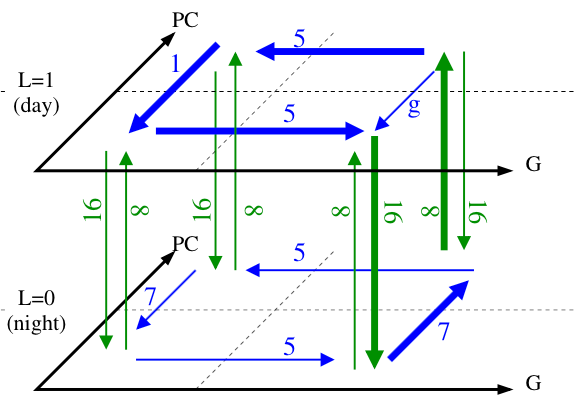
\includegraphics[width=1\textwidth]{Delayed1.png}
\caption*{(a)}
\end{minipage}
\begin{minipage}{0.4\linewidth}
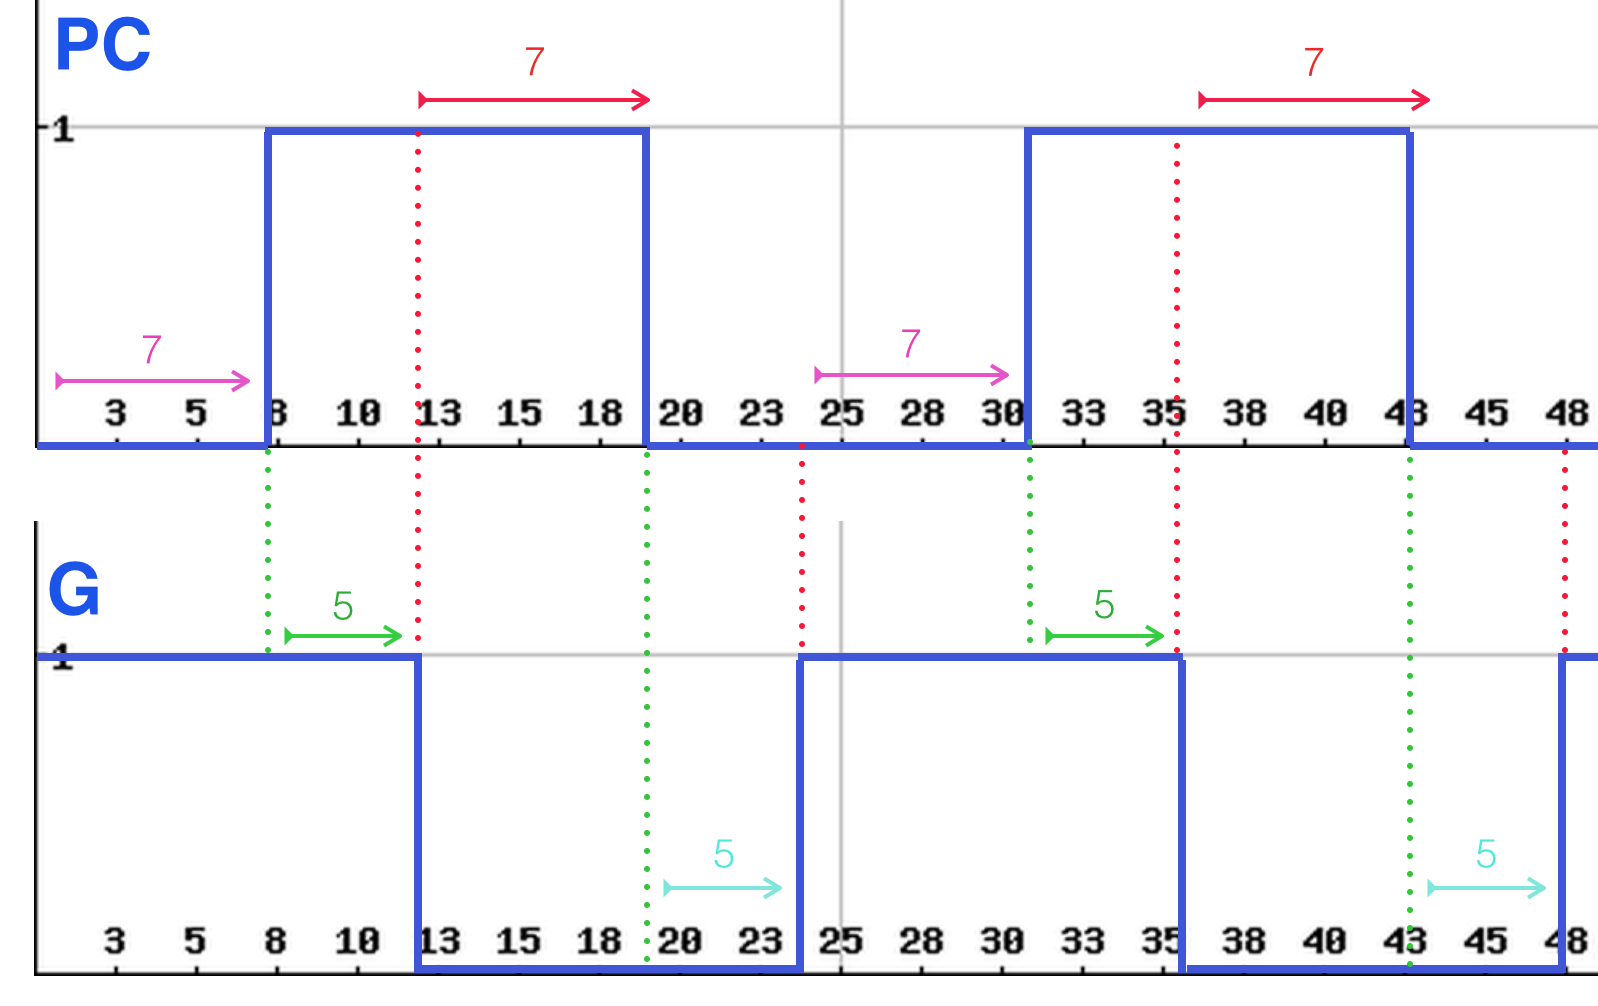
\includegraphics[width=1\textwidth]{Delayed2.png}
\caption*{(b)}
\end{minipage}
\caption{(a) le mod\`ele qualitatif de cycle circadien mammalien pendant l'\'et\'e (b) le chronogramme correspondant \`a la discr\'etisation des donn\'ees d'observation des processus pendant la nuit ($L=0$).}\label{mammal}
\end{figure}
Selon Algorithme \ref{sysret}, 10 actions sont g\'en\'er\'ees : 

\begin{table}[ht]
\centering
\begin{tabular}{|c|c|}
\hline 
$\{L_0\}\stackrel{8}{\to}L_0\Rsh L_1$ & $\{L_1\}\stackrel{16}{\to}L_1\Rsh L_0$ \\ 
\hline 
$\{L_0,G_0\}\stackrel{7}{\to}PC_1\Rsh PC_0$ & $\{L_0,PC_0\}\stackrel{5}{\to}G_0\Rsh G_1$ \\ 
\hline 
$\{L_0,G_1\}\stackrel{7}{\to}PC_0\Rsh PC_1$ & $\{L_0,PC_1\}\stackrel{5}{\to}G_1\Rsh G_0$ \\ 
\hline 
$\{L_1,G_0\}\stackrel{7}{\to}PC_1\Rsh PC_0$ & $\{L_1,PC_0\}\stackrel{5}{\to}G_0\Rsh G_1$ \\ 
\hline 
$\{L_1,G_1\}\stackrel{7}{\to}PC_1\Rsh PC_0$ & $\{L_1,PC_1\}\stackrel{5}{\to}G_1\Rsh G_0$ \\ 
\hline 
\end{tabular} 
\end{table}
qui v\'erifie et enrichit la s\'emantique du r\'eseau de r\'egulation dans Figure \ref{mammalpic} :

\begin{figure}[ht]
\centering
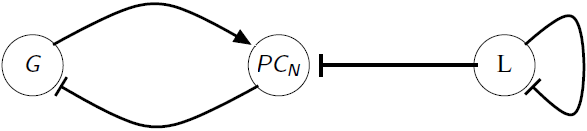
\includegraphics[scale=0.6]{mammal.png}
\caption{Le graphe de r\'egulation simplifi\'e du mod\`ele de cycle circadien mammalien}\label{mammalpic}
\end{figure}

\end{document}